\documentclass[12pt,a4paper,openright,fontset=windows]{ctexbook}

% ======================
% 编译方式：XeLaTeX
% ======================
\usepackage{fontspec}

% 英文字体
\setmainfont{Times New Roman}
\setsansfont{Arial}

% 中文字体
\setCJKmainfont{SimSun}        % 宋体
\setCJKsansfont{SimHei}        % 黑体
\setCJKmonofont{FangSong}      % 仿宋

% ======================
% 页面设置
% ======================
\usepackage{geometry}
\geometry{
    a4paper,
    top=3cm,
    bottom=3cm,
    left=3cm,
    right=3cm
}

% ======================
% 基础宏包
% ======================
\usepackage{amsmath, amssymb}
\usepackage{graphicx}
\usepackage{booktabs}
\usepackage{array}
\usepackage{float}
\usepackage{caption}
\usepackage{subcaption}
\usepackage{setspace}
\usepackage{indentfirst}
\usepackage{titlesec}
\usepackage{tocloft}
\usepackage{fancyhdr}
\usepackage[numbers,sort&compress,super]{natbib}
\usepackage{hyperref}

% ======================
% 正文段落格式
% ======================
\setlength{\parindent}{2em}
\setlength{\parskip}{0pt}
\linespread{1.38}

% ======================
% 页眉页码
% ======================
\pagestyle{fancy}
\fancyhf{}
\renewcommand{\headrulewidth}{0pt}
\fancyfoot[C]{\thepage}

% ======================
% 章节标题格式
% ======================

% 章标题：黑体三号，居中，段前24磅，段后18磅
\titleformat{\chapter}
  {\centering\heiti\fontsize{16pt}{20pt}\selectfont}
  {第\,\thechapter\,章}
  {1em}
  {}

\titlespacing*{\chapter}
  {0pt}
  {24pt}
  {18pt}

% 一级节标题：黑体四号，居左，段前24磅，段后6磅
\titleformat{\section}
  {\heiti\fontsize{14pt}{20pt}\selectfont}
  {\thesection}
  {1em}
  {}

\titlespacing*{\section}
  {0pt}
  {24pt}
  {6pt}

% 二级节标题：黑体13pt，居左，段前12磅，段后6磅
\titleformat{\subsection}
  {\heiti\fontsize{13pt}{20pt}\selectfont}
  {\thesubsection}
  {1em}
  {}

\titlespacing*{\subsection}
  {0pt}
  {12pt}
  {6pt}

% 三级节标题：黑体小四，居左，段前12磅，段后6磅
\titleformat{\subsubsection}
  {\heiti\fontsize{12pt}{20pt}\selectfont}
  {\thesubsubsection}
  {1em}
  {}

\titlespacing*{\subsubsection}
  {0pt}
  {12pt}
  {6pt}

% ======================
% 图表格式
% ======================
\renewcommand{\figurename}{图}
\renewcommand{\tablename}{表}

\captionsetup[figure]{
    font={small},
    labelfont={normalfont},
    labelsep=space,
    justification=centering,
    skip=6pt,
    position=bottom
}

\captionsetup[table]{
    font={small},
    labelfont={normalfont},
    labelsep=space,
    justification=centering,
    skip=6pt,
    position=top
}

% 图、表、公式按章编号
\numberwithin{figure}{chapter}
\numberwithin{table}{chapter}
\numberwithin{equation}{chapter}

% ======================
% 目录格式
% ======================
\renewcommand{\contentsname}{目录}
\setcounter{tocdepth}{1}

\renewcommand{\cftchapfont}{\heiti\fontsize{12pt}{20pt}\selectfont}
\renewcommand{\cftchappagefont}{\fontsize{12pt}{20pt}\selectfont}

\renewcommand{\cftsecfont}{\songti\fontsize{12pt}{20pt}\selectfont}
\renewcommand{\cftsecpagefont}{\fontsize{12pt}{20pt}\selectfont}

\renewcommand{\cftsubsecfont}{\songti\fontsize{12pt}{20pt}\selectfont}
\renewcommand{\cftsubsecpagefont}{\fontsize{12pt}{20pt}\selectfont}

% ======================
% 超链接设置
% ======================
\hypersetup{
    colorlinks=true,
    linkcolor=black,
    citecolor=black,
    urlcolor=black
}

% ======================
% 图片路径
% ======================
\graphicspath{{figures/}}

\begin{document}

% ======================
% 目录
% ======================
\pagenumbering{Roman}
\tableofcontents
\cleardoublepage

% ======================
% 正文
% ======================
\pagenumbering{arabic}

\chapter{绪论}

\section{研究背景及意义}

气候变化已经成为全球能源系统转型必须面对的长期约束。为控制温室气体排放，《巴黎协定》提出将全球平均气温升幅控制在较工业化前水平明显低于 \(2\,^\circ\mathrm{C}\) 的范围内，并努力限制在 \(1.5\,^\circ\mathrm{C}\) 以内\cite{unfccc_paris_2015}。中国作为全球重要能源消费国和制造业大国，提出力争于 2030 年前实现二氧化碳排放达峰、2060 年前实现碳中和\cite{china_ndc_2021}。在这一目标牵引下，电力系统需要在保障供电安全的同时持续降低单位电量碳排放，能源结构也正由以煤电为主体的传统形态向高比例可再生能源与多元调节资源协同的新型电力系统转变。

风电、光伏等可再生能源具有清洁低碳优势，但其出力受气象条件影响显著，存在波动性、间歇性和预测误差。随着新能源装机占比提升，电力系统对灵活调节电源、快速爬坡能力和备用容量的需求同步增加。燃气轮机及燃气-蒸汽联合循环机组具有启停速度快、负荷调节范围宽、单位发电碳排放低于常规燃煤机组、污染物排放控制相对容易等特点，能够在新能源消纳、电网调峰、冷热电联供和应急备用等场景中发挥重要作用。国际能源署等机构也指出，在高比例可再生能源系统中，灵活可调的低排放电源和储能、需求响应等资源共同构成系统安全运行的重要支撑\cite{iea_weo_2023}。因此，在较长时期内，燃气机组并不是简单的过渡性设备，而是连接化石能源清洁利用、可再生能源大规模接入和电力系统可靠运行的关键装备。

燃气-蒸汽联合循环机组通过燃气轮机布雷顿循环与蒸汽朗肯循环的耦合，实现燃料化学能的梯级利用，具有较高的热效率和较好的工程成熟度。典型联合循环系统中，燃气轮机排出的高温烟气进入余热锅炉产生蒸汽，并进一步推动汽轮机做功，从而提高系统总出力和燃料利用效率。其基本流程如图 \ref{fig:chapter1-ccpp-schematic} 所示。与单一循环相比，联合循环系统内部包含压气机、燃烧室、燃气透平、余热锅炉、汽轮机、凝汽器、给水系统和热网抽汽等多个相互耦合的设备，热力过程跨越气体侧和汽水侧，运行性能受环境条件、燃料组成、负荷水平、设备退化和控制策略等多重因素共同影响。

\begin{figure}[!htb]
  \centering
  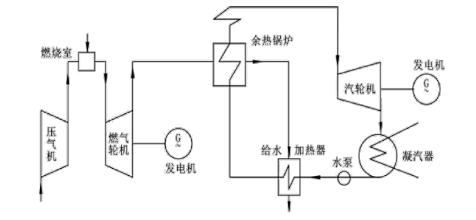
\includegraphics[width=0.86\textwidth]{chapter1/燃气蒸汽联合循环示意图.png}
  \caption{燃气-蒸汽联合循环系统示意图}
  \label{fig:chapter1-ccpp-schematic}
\end{figure}

在工程运行中，燃气机组往往长期处于偏离设计工况的状态。一方面，电网调峰和供热需求使机组频繁经历部分负荷、启停和变负荷运行；另一方面，环境温度、压力、湿度和燃料组分的变化会改变压气机进气条件、燃烧过程和余热回收特性；此外，设备长期运行还会引起压气机污垢、透平通流能力变化、余热锅炉换热性能下降、汽轮机通流部分结垢等退化现象。这些因素会使压比、空气流量、透平排气温度、蒸汽参数、真空度和机组效率等关键指标偏离设计值，导致运行状态、能量分配和经济性发生变化。若仍以设计工况或静态经验指标评价机组性能，容易掩盖工况变化与设备退化的差异，也难以为高效可靠运行提供可靠依据。

因此，有必要面向真实运行数据重新评估燃气-蒸汽联合循环机组的运行状态，建立能够反映多工质、多设备和变工况特征的热力分析方法。通过对实测数据进行工质状态构造、设备能量分析和关键参数影响分析，可以识别机组在实际运行中的能量转换规律和主要损失环节，区分环境扰动、负荷变化和设备性能变化对效率的影响，为运行人员开展参数调整、负荷分配、维护决策和节能降耗提供定量依据。这不仅有助于提高单台机组的运行经济性，也能够在更大尺度上支撑新型电力系统低碳、安全和灵活运行。

\section{国内外研究现状}

燃气-蒸汽联合循环机组性能研究首先依赖于对系统热力过程的合理描述。现有研究通常以压气机、燃烧室、燃气透平、余热锅炉、汽轮机和凝汽器等关键设备为对象，基于质量守恒、能量守恒、部件特性关系和换热关系建立系统级热力模型。早期气路分析方法以燃气轮机部件性能偏差识别为核心，为后续燃气轮机状态评估和性能诊断奠定了基础\cite{urban1973gpa,stamatis2011gpa,fentaye2019review}；压气机和燃气透平特性建模则通过通用特性、变工况修正和参数校正等方法，为部件级性能计算提供支撑\cite{zhang1996compressor,lu1996turbine,volponi1999corrections}。面向工程应用的研究进一步将机理模型、现场测量和健康监测结合起来，用于燃气轮机性能评估、诊断和预测性维护\cite{tahan2017health,hanachi2018survey}。对于联合循环机组而言，这类模型能够把燃气轮机侧的布雷顿循环与汽水侧的朗肯循环联系起来，适合分析负荷变化、环境条件变化和设备边界条件变化对机组效率、出力和热耗率的影响。近年来，面向实际机组的模块化热力建模和运行数据修正逐渐成为提高模型工程适用性的重要方法\cite{wang2023hrsg,tsoutsanis2014map,ying2023diagnostic}。

在性能影响因素方面，国内外研究均指出联合循环机组效率不是单一参数决定的结果，而是负荷、环境条件、燃气轮机运行参数和蒸汽循环边界条件共同作用的结果。对于燃气轮机侧，环境温度、环境压力、进气流量、燃料流量、压气机压比和透平入口温度会影响压气机耗功、燃烧室出口状态、透平输出功和排气余热；对于蒸汽循环侧，余热锅炉换热过程、主蒸汽流量与压力、凝汽器真空度以及供热抽汽条件会影响汽轮机出力和全厂能量利用水平。已有研究从部分负荷特性、不同控制策略和环境温度影响等角度分析了联合循环变工况性能，指出燃气轮机与蒸汽循环之间存在明显耦合，系统性能需要从全厂角度评价\cite{kim2004partload,hyun2018dual,yang2019inlet,zhang2018chp,li2018backpressure}。同时，多压力联合循环、余热锅炉参数和蒸汽压力等因素也会影响烟气余热回收效率和底循环出力\cite{ibrahim2014multipressure,yang2018hrsg,liying2006steam}。因此，机组在部分负荷和变环境条件下常常偏离设计工况，需要从燃气轮机、余热锅炉和汽轮机之间的能量传递关系出发分析参数影响，而不能只考察单一设备或单一效率指标。本文后续对环境参数、燃机出力、汽机出力、给水压力、主蒸汽流量和供热量等变量的分析，正是沿着这一研究方向展开。

随着燃气机组承担更多调峰和灵活运行任务，长期宽工况运行下的状态评估逐渐成为研究重点。燃气轮机在长期运行中会受到积垢、腐蚀、磨损和热疲劳等因素影响，导致部件效率、通流能力和排气状态逐渐偏离设计基准\cite{diakunchak1992deterioration,kurz2001degradation}。联合循环系统中，燃气轮机、余热锅炉和汽轮机性能变化还会通过排气温度、烟气流量和蒸汽参数相互传递，从而影响全厂效率和负荷分配；余热锅炉换热面结垢、汽轮机通流部分退化等问题也会改变底循环吸热和做功过程\cite{marner1984fouling,zwebek2003degradation,massardo2009hrsg}。已有退化和性能诊断研究表明，若不能区分环境扰动、工况变化与设备性能变化，容易将正常变工况影响误判为设备退化\cite{li2009prognostic,tahan2017health}，因此需要通过实测数据重新构造机组运行状态，进行设备性能评估。

实际生产数据还存在测点不完整、关键参数难以直接测量和设备状态难以准确标注等问题。现场性能试验和能量监测研究指出，流量、温度、压力等测量量的不确定性会直接影响燃气轮机和联合循环性能计算结果\cite{pinelli2000uncertainties,carstens2018uncertainty}；同时，燃烧室出口温度、部分流量和湿蒸汽状态等关键参数往往难以直接测得，设备特性曲线和内部结构参数也可能因商业保密或现场条件限制而不完备\cite{colera2019thermodynamic,vonmoll2014egt,vemulapalli2022softsensor,tian2018softmeasurement}。这些问题说明，在真实联合循环机组上开展性能分析时，应尽量利用已有测点建立统一的工质状态和设备平衡关系，并通过数据一致性检查提高分析结果的可信度。

除能量分析外，㶲分析也被广泛用于联合循环系统性能评价。㶲分析以热力学第二定律为基础，能够进一步揭示不同设备中的不可逆损失和能量品质下降位置。已有研究将㶲分析与参数优化、多目标优化和环境经济评价相结合，用于识别燃烧室、余热锅炉、透平等设备的主要损失来源，并分析压比、透平入口温度、蒸汽参数等变量对系统性能的影响\cite{kaviri2012exergy,ahmadi2011exergo}。这类研究说明，仅从能量守恒角度分析联合循环机组仍不够充分，还需要结合㶲效率和㶲损失评价不同能量流的可用能水平。本文在实测数据基础上建立了包含㶲计算的统一流股模型，为后续进一步开展㶲分析预留了接口。受数据条件和研究周期限制，本文以能量分析为主线，重点从热力学第一定律角度刻画真实机组的能量利用过程。

\section{研究内容与章节安排}

本文以某燃气-蒸汽联合循环机组为研究对象，所用数据来自该机组 2025 年 4 月至 12 月的实际运行记录。数据覆盖燃气轮机、余热锅炉、汽轮机、凝汽器和热网抽汽等主要系统，包含环境参数、工质参数、部件参数等相关变量。由于该数据来源于生产现场，其工况分布并非理想设计点附近的少量稳态样本，而是包含季节变化、负荷调节、供热需求变化和设备状态波动的长期运行数据。因此，本文研究具有较强的工程真实性，也要求模型能够处理变工况、多变量和多设备耦合问题。

围绕上述对象，本文主要开展以下研究工作。第一，建立联合循环机组多工质流股建模方法。针对燃料气、湿空气、烟气、水和水蒸气等不同工质，构造统一的流股对象，计算温度、压力、质量流量、比焓、比熵、能量流和㶲流等状态量，为后续设备模型提供一致的数据接口。第二，建立燃气轮机、余热锅炉和汽轮机等关键设备的热力分析模型。基于热力学定律计算各设备的能量输入输出、功率分配、换热特性、能量损失和效率指标，从设备级揭示实际运行中的性能变化规律。第三，结合真实运行数据分析联合循环机组关键运行参数对性能的影响。通过对环境温度、环境压力、环境湿度、燃机出力、汽机出力、供热量、给水压力、主蒸汽流量和透平排气温度等变量进行相关性和散点规律分析，识别影响整机效率的主要因素，为运行诊断和性能评估提供依据。本文的研究建立了基于燃气-蒸汽联合循环机组的热力分析模型，为机组运行状态评估和效率分析奠定基础。

全文章节安排如下。

第 1 章为绪论，介绍低碳能源转型背景下燃气-蒸汽联合循环机组的重要作用，总结国内外关于性能评估和退化识别的研究现状，并说明本文研究内容与数据来源。

第 2 章介绍联合循环机组工质建模方法，建立燃料气、湿空气、烟气、水和水蒸气的物性计算与统一流股描述方法，并给出由实测数据构造全厂流股对象的过程。

第 3 章建立燃气轮机侧性能分析模型，围绕压气机、燃烧室和燃气透平等部件开展能量分析，研究燃气轮机在实际运行数据下的状态变化。

第 4 章建立余热锅炉和汽轮机侧热力分析模型，分析烟气余热利用、汽水侧吸热、汽轮机出力分配和相关效率指标。

第 5 章基于实际运行数据开展机组性能影响因素分析，结合相关性矩阵和关键变量散点关系，识别影响整机效率的主要运行参数。

第 6 章总结全文研究结论，归纳本文工作的主要认识，并对后续在线状态评估和模型扩展方向进行展望。

\chapter{工质建模方法}

\section{联合循环机组工质建模对象与总体思路}

联合循环机组由气体循环和蒸汽循环耦合构成，机组内部同时存在燃料气、空气、燃烧产物烟气、水以及水蒸气等多类工质。不同工质在热力性质、组分、状态确定方式以及能量转换方面存在明显差异。燃气轮机侧主要涉及气体混合物的压缩、燃烧和膨胀过程，余热锅炉和汽水系统侧则主要涉及水和水蒸气的加压、加热、蒸发、过热、膨胀和凝结过程。因此，在建立联合循环机组能量分析与火用分析模型之前，有必要首先建立统一、清晰且可复用的工质流股建模方法，为后续压气机、燃烧室、燃气透平、余热锅炉、汽轮机和凝汽器等设备模型提供统一的工质输入和输出接口。

本文的工质建模方法以流股为基本对象，首先需要确定各类工质的状态参数。对于水和水蒸气工质，其状态通常由两个独立状态参数确定。常用输入组合包括压力和温度 $(P,T)$、压力和干度 $(P,x)$、压力和比焓 $(P,h)$ 以及压力和比熵 $(P,s)$。对于气体工质，在上述两个独立状态参数的基础上还需要考虑气体组分。因此，工质状态建模的核心是根据不同输入组合确定其余参数，为后续分析提供基础。

联合循环机组性能分析涉及多个设备和多种工质。为了保证不同设备模型之间能够稳定传递状态信息，工质状态模型需要满足统一性、可扩展性等要求。因此分别采用本文采用 IAPWS-IF97 物性库计算水和水蒸气的热力性质，采用 CoolProp 开源物性库辅助计算气体工质的热力性质。在气体工质物性计算中，本文以标准状态作为基准状态，即
\[
T_{\mathrm{ref}}=273.15\,\mathrm{K}, \qquad
P_{\mathrm{ref}}=101325\,\mathrm{Pa}.
\]
在该基准状态下定义混合气的基准比焓和基准比熵。

在流股的封装方面，本文在程序实现中将工质模块划分为统一流股状态、气体工质、水和水蒸气工质、参考环境以及实测数据流股构造等部分。其核心思想是：先由基础物性模型计算单个工质状态，再将状态封装为统一的流股对象，最后将流股对象作为设备模型的输入和输出。通过该方法，可以使联合循环机组中不同设备之间的工质状态传递具有统一的数据结构和接口形式，从而提高模型的可读性、可维护性和工程适用性，为后续的自动化建模和数据驱动的建模提供了坚实的基础。

\section{流股状态的统一描述方法}

在联合循环机组中，工质在不同设备之间以流股形式传递。无论是进入压气机的空气、进入燃烧室的燃料气、流经燃气透平和余热锅炉的烟气，还是汽水系统中的给水、饱和水、饱和蒸汽和过热蒸汽，本质上都可以看作携带质量、能量和火用的流动介质。为了避免不同设备模型之间重复定义状态参数，本文采用统一流股对象对各类工质状态进行描述。

统一流股对象的核心思想是：将工质的质量流量、温度、压力、比焓、比熵、组成、能量流率和火用流率等参数封装为同一类状态对象，并将其作为设备模型的输入和输出。这样可以使压气机、燃烧室、燃气透平、余热锅炉、汽轮机和凝汽器等设备模型采用一致的接口形式，从而提高模型的可读性和可扩展性。

对于任一流股 $k$，其状态可表示为
\[
\mathcal{F}_k
=
\left\{
\dot{m}_k,\,
T_k,\,
P_k,\,
h_k,\,
s_k,\,
\boldsymbol{x}_k,\,
e_{x,k},\,
\right\},
\]
其中，$\dot{m}_k$ 为质量流量，$T_k$ 为温度，$P_k$ 为压力，$h_k$ 为比焓，$s_k$ 为比熵，$\boldsymbol{x}_k$ 为组分，$e_{x,k}$ 为比火用。其中，比焓 $h_k$ 反映单位质量工质所携带的热力学能量，比熵 $s_k$ 则用于描述工质状态变化的不可逆性和火用水平。基于此可以计算比火用 $e_{x,k}$。若以参考环境为基准，比火用可表示为
\[
e_{x,k}
=
\left(h_k-h_{0,k}\right)
-
T_0\left(s_k-s_{0,k}\right),
\]
其中，$T_0$ 为环境参考温度，$h_{0,k}$ 和 $s_{0,k}$ 分别为第 $k$ 条流股对应工质在参考环境下的比焓和比熵。

联合循环机组的性能分析通常包括能量分析和火用分析两个层次。能量分析以热力学第一定律为基础，重点关注能量在不同设备之间的传递与转换；火用分析以热力学第二定律为基础，重点关注能量品质和不可逆损失。因此，在流股状态建模中，需要同时建立能量流和火用流的统一表达。

对于任一流股，其焓流率可表示为
\[
\dot{H}
=
\dot{m}h.
\]

对于具有多个入口和出口的稳态设备，忽略动能和位能变化时，其能量平衡方程可写为
\[
\dot{Q}
-
\dot{W}
+
\sum_{\mathrm{in}}\dot{m}_{\mathrm{in}}h_{\mathrm{in}}
-
\sum_{\mathrm{out}}\dot{m}_{\mathrm{out}}h_{\mathrm{out}}
=
0,
\]
其中，$\dot{Q}$ 为设备与外界的换热量，$\dot{W}$ 为设备对外输出的功。若设备为压气机或泵，则通常表现为外界对设备输入功；若设备为燃气透平或汽轮机，则表现为设备对外输出功。

火用流反映的是流股相对于参考环境所具有的最大理论做功能力。对于不考虑动能和位能的流股，其物理比火用为
\[
e_x
=
\left(h-h_0\right)
-
T_0\left(s-s_0\right).
\]
对应的火用流率为
\[
\dot{E}_x
=
\dot{m}
\left[
\left(h-h_0\right)
-
T_0\left(s-s_0\right)
\right].
\]

若进一步考虑流股动能和位能，则总比火用可写为
\[
e_{x,\mathrm{tot}}
=
\left(h-h_0\right)
-
T_0\left(s-s_0\right)
+
\frac{c^2}{2}
+
gz,
\]
其中，$c$ 为流速，$g$ 为重力加速度，$z$ 为高度。对于本文所研究的联合循环机组热力系统，设备进出口高度差和流速变化对整体能量分析影响较小，因此可以忽略不计。

对于稳态开口系统，火用平衡方程可表示为
\[
\sum_{\mathrm{in}}\dot{E}_{x,\mathrm{in}}
-
\sum_{\mathrm{out}}\dot{E}_{x,\mathrm{out}}
+
\sum_j
\left(
1-\frac{T_0}{T_j}
\right)
\dot{Q}_j
-
\dot{W}
=
\dot{E}_{x,\mathrm{dest}},
\]
其中，$T_j$ 为第 $j$ 个换热边界温度，$\dot{Q}_j$ 为通过该边界传递的热量，$\dot{E}_{x,\mathrm{dest}}$ 为火用损失率。根据 Gouy--Stodola 定理，火用损失与熵产之间满足
\[
\dot{E}_{x,\mathrm{dest}}
=
T_0\dot{S}_{\mathrm{gen}},
\]
其中，$\dot{S}_{\mathrm{gen}}$ 为设备内部不可逆过程产生的熵产率。

对于绝热设备，若忽略与外界的换热，则火用平衡可简化为
\[
\sum_{\mathrm{in}}\dot{E}_{x,\mathrm{in}}
-
\sum_{\mathrm{out}}\dot{E}_{x,\mathrm{out}}
-
\dot{W}
=
\dot{E}_{x,\mathrm{dest}}.
\]
对于透平，设备输出功 $\dot{W}_{\mathrm{out}}$ 可由入口和出口火用差扣除火用损失得到：
\[
\dot{W}_{\mathrm{out}}
=
\dot{E}_{x,\mathrm{in}}
-
\dot{E}_{x,\mathrm{out}}
-
\dot{E}_{x,\mathrm{dest}}.
\]
对于压气机或泵，输入功则可表示为
\[
\dot{W}_{\mathrm{in}}
=
\dot{E}_{x,\mathrm{out}}
-
\dot{E}_{x,\mathrm{in}}
+
\dot{E}_{x,\mathrm{dest}}.
\]

由上述表达可知，统一流股对象中的 $h$ 和 $s$ 是连接能量分析与火用分析的关键参数。比焓决定流股携带的能量水平，比熵与参考环境共同决定流股的可用能水平。通过在流股对象中统一定义 $\dot{H}$、$e_x$ 和 $\dot{E}_x$，可以避免在不同设备模型中重复编写能量流和火用流计算公式。

统一流股对象是本文联合循环机组建模方法中的基础环节。它一方面向下连接气体和水蒸气的物性计算方法，另一方面向上支撑各类设备模型和系统性能分析模型。通过该方法，可以使复杂联合循环机组中的多工质、多设备、多状态点问题转化为一组标准化流股对象之间的变换关系，从而提高模型的结构清晰度和工程适用性。

\section{气体工质组成与物性建模方法}

\subsection{燃料气组成表示与归一化处理}

燃料气组成是气体工质建模的基础输入之一。对于燃气轮机系统而言，燃料气并非单一组分，而是由氢气、甲烷、乙烷、一氧化碳、二氧化碳、氮气以及少量高碳烃类共同组成。不同组分的摩尔质量、低位发热量以及热力性质均存在明显差异，因此在进行燃料热值、烟气生成量、混合气焓熵和火用计算之前，需要首先建立统一的燃料气组成表示方法。

CoolProp 物性库是一个开源数据库，提供了多种纯组分和混合物的热力性质计算接口。本文程序利用 CoolProp 查询燃料气中各组分的摩尔质量、低位发热量以及热力性质等参数。为了保证后续计算的一致性，程序预设了一个固定的燃料组分列表，并要求输入数据中的燃料组成必须包含该列表中的所有组分。

气体组分可以表示为各组分的摩尔分数，主要包括
\[
\mathrm{H_2},\ \mathrm{N_2},\ \mathrm{CO_2},\ \mathrm{CH_4},\ \mathrm{CO},\ \mathrm{O_2},\ \mathrm{H_2O},
\mathrm{C_2H_6},\ \mathrm{C_3H_8},\ i\mathrm{C_4H_{10}},\ n\mathrm{C_4H_{10}},
i\mathrm{C_5H_{12}},\ n\mathrm{C_5H_{12}} .
\]
其中，氢气、甲烷、一氧化碳以及 C2--C5 烃类为主要可燃组分，氮气、二氧化碳和氧气等则作为燃料中的惰性组分参与混合物平均性质计算。程序通过固定组分列表保证后续物性计算、燃烧产物计算和低位发热量计算使用一致的组分顺序与组分名称。

由于原始组分数据可能未严格归一化，程序在使用燃料组成前均进行归一化处理。设原始输入中第 \(i\) 种组分的相对含量为 \(y_i\)，则归一化后的摩尔分数 \(x_i\) 为
\[
x_i = \frac{y_i}{\sum_{j=1}^{N} y_j},
\]
其中 \(N\) 为参与建模的气体组分数。归一化处理后，燃料气平均摩尔质量可由各组分摩尔分数加权得到：
\[
M_{\mathrm{mix}} = \sum_{i=1}^{N} x_i M_i,
\]
式中，\(M_i\) 为第 \(i\) 种纯组分的摩尔质量。各纯组分摩尔质量由 CoolProp 物性库查询获得。

\subsection{湿空气组成计算方法}

燃气轮机入口空气是燃烧过程的重要反应物，其组成直接影响燃烧所需氧量、烟气生成量以及压气机和余热锅炉烟气侧的热力性质计算。实际环境空气并非完全干空气，而是含有一定水蒸气的湿空气。环境湿度变化会改变空气中氧气和氮气的有效摩尔分数，并进一步影响燃烧产物中水蒸气含量和烟气平均摩尔质量。因此，在构造燃气轮机入口空气流股时，需要根据环境温度、压力和相对湿度对空气组成进行修正。

首先将干空气视为由氧气、氮气和少量二氧化碳组成的混合气体，其基准摩尔分数取为
\[
x_{\mathrm{O_2,dry}} = 0.2095,\quad
x_{\mathrm{N_2,dry}} = 0.7808,\quad
x_{\mathrm{CO_2,dry}} = 0.0004 .
\]
该组成用于表示进入压气机前的干空气主体成分。由于氩气等微量组分在本文模型中未单独建立物性计算项，其影响在工程计算中近似并入主要惰性组分处理。

湿空气中的水蒸气摩尔分数由环境相对湿度计算。程序中首先调用 CoolProp 根据环境温度 \(T\) 计算水的饱和蒸气压 \(p_{\mathrm{sat}}(T)\)，再由相对湿度 \(RH\) 和环境压力 \(P\) 得到水蒸气分压：
\[
p_{\mathrm{H_2O}} = \varphi p_{\mathrm{sat}}(T),
\]
其中，\(\varphi\) 为相对湿度的小数形式。根据理想气体混合物中摩尔分数等于分压占总压的比例，湿空气中水蒸气摩尔分数可表示为
\[
x_{\mathrm{H_2O}} = \frac{p_{\mathrm{H_2O}}}{P}
=
\frac{\varphi p_{\mathrm{sat}}(T)}{P}.
\]

得到水蒸气摩尔分数后，干空气中各组分的摩尔分数按剩余气相比例进行缩放：
\[
x_{i,\mathrm{wet}} = x_{i,\mathrm{dry}}\left(1-x_{\mathrm{H_2O}}\right),
\quad
i \in \{\mathrm{O_2},\mathrm{N_2},\mathrm{CO_2}\}.
\]
同时令
\[
x_{\mathrm{H_2O,wet}} = x_{\mathrm{H_2O}}.
\]
由此可得湿空气组成：
\[
\boldsymbol{x}_{\mathrm{air}}
=
\left[
x_{\mathrm{O_2,wet}},
x_{\mathrm{N_2,wet}},
x_{\mathrm{CO_2,wet}},
x_{\mathrm{H_2O,wet}}
\right].
\]
随后将该组成转换为统一的气体组成对象，并再次归一化，以消除数值舍入或输入误差对组分总和的影响。

在本文模型中，湿空气组成主要用于两个方面。一方面，入口空气作为燃气轮机压气机工质，需要根据其组成计算焓、熵、定压比热和气体常数等热力性质；另一方面，空气中的氧气、水蒸气和惰性组分会进入燃烧产物计算，决定余热锅炉入口烟气的组成和物性。通过将相对湿度引入空气组成建模，程序能够反映环境条件变化对燃气轮机入口工质和烟气侧热力计算的影响，从而提高不同运行工况下性能分析结果的一致性。

\subsection{燃烧产物与烟气组成计算方法}

燃烧产物组成是燃气轮机排气和余热锅炉烟气侧热力计算的基础。燃料气与空气在燃烧室内反应后，燃料中的可燃组分被氧化生成二氧化碳和水蒸气，空气中的氮气以及燃料中的惰性组分则随烟气进入余热锅炉。烟气组成不仅决定混合气平均摩尔质量，也会影响烟气焓、熵、定压比热、密度以及火用计算结果。因此，在构造烟气流股之前，需要根据燃料组成、空气组成以及二者的质量流量计算燃烧产物组成。

首先利用燃料气和空气的平均摩尔质量，将质量流量换算为摩尔流量：
\[
\dot{n}_{\mathrm{fuel}}
=
\frac{\dot{m}_{\mathrm{fuel}}}{M_{\mathrm{fuel}}},
\qquad
\dot{n}_{\mathrm{air}}
=
\frac{\dot{m}_{\mathrm{air}}}{M_{\mathrm{air}}}.
\]
式中，\(\dot{m}_{\mathrm{fuel}}\) 和 \(\dot{m}_{\mathrm{air}}\) 分别为燃料和空气质量流量，\(M_{\mathrm{fuel}}\) 和 \(M_{\mathrm{air}}\) 分别为燃料气和湿空气平均摩尔质量。

在燃烧反应计算中，程序对燃料中的主要含碳组分和含氢组分分别建立化学计量关系。对于碳元素，甲烷、一氧化碳、乙烷、丙烷、丁烷和戊烷等组分完全燃烧后生成二氧化碳。若第 \(k\) 种燃料组分的摩尔分数为 \(x_k\)，其分子中碳原子数为 \(a_k\)，则由燃料燃烧生成的二氧化碳摩尔流量可表示为
\[
\dot{n}_{\mathrm{CO_2,prod}}
=
\dot{n}_{\mathrm{fuel}}
\sum_k x_k a_k .
\]
对于氢元素，氢气和各烃类燃烧生成水蒸气。若第 \(k\) 种组分完全燃烧生成水蒸气的化学计量系数为 \(b_k\)，则燃烧生成的水蒸气摩尔流量为
\[
\dot{n}_{\mathrm{H_2O,prod}}
=
\dot{n}_{\mathrm{fuel}}
\sum_k x_k b_k .
\]
通过给出各可燃组分对应的碳原子数、水蒸气生成系数和理论需氧系数，将燃烧反应计算转化为统一的组分加权求和。

根据燃烧反应对各组分摩尔流量进行计算后，程序将烟气组分总量归一化，得到烟气摩尔分数组成：
\[
x_{i,\mathrm{flue}}
=
\frac{\dot{n}_{i,\mathrm{flue}}}
{\sum_j \dot{n}_{j,\mathrm{flue}}}.
\]

该方法能够利用运行数据中的燃料流量、空气流量和燃料组分推算余热锅炉入口烟气组成，并为后续烟气焓熵计算、烟气密度计算和余热利用分析提供统一的气体组成输入。

\subsection{混合气体工质的物性计算}

在确定燃料气、湿空气和烟气组成后，需要进一步计算混合气体的焓、熵、定压比热以及气体常数等热力性质，可根据各组分摩尔分数对纯组分物性进行加权，得混合气体的物性。

对于给定温度 \(T\)、压力 \(P\) 和组成 \(\boldsymbol{x}\)，首先对气体组成进行归一化处理，然后遍历所有组分。对于第 \(i\) 种组分，其摩尔分数为 \(x_i\)，程序采用理想气体混合物分压关系计算该组分分压：
\[
p_i = x_i P .
\]
在此基础上，调用纯组分物性计算函数获得该组分在 \(T\)、\(p_i\) 下的摩尔焓 \(h_i^{\mathrm{m}}\)、摩尔熵 \(s_i^{\mathrm{m}}\) 和摩尔定压比热 \(c_{p,i}^{\mathrm{m}}\)。

利用 CoolProp 查询气体纯组分的摩尔质量、摩尔焓、摩尔熵和摩尔定压比热等参数：

\[
h_i^{\mathrm{m}} = h_i^{\mathrm{m}}(T,p_i),\quad
s_i^{\mathrm{m}} = s_i^{\mathrm{m}}(T,p_i),\quad
c_{p,i}^{\mathrm{m}} = c_{p,i}^{\mathrm{m}}(T,p_i).
\]

对于燃料气、空气和烟气中的氢气、氮气、二氧化碳、甲烷、一氧化碳、氧气以及部分烃类组分，通过物性库在给定温度和压力下获取纯组分物性，再完成摩尔分数加权。

对于烟气中的水蒸气，为防止相变取数据库无法处理的问题，采用 Shomate 方程计算其理想气体热力性质。Shomate 方程以温度多项式形式给出水蒸气的摩尔焓、摩尔熵和摩尔定压比热，适用于燃气轮机和余热锅炉烟气侧较宽的温度范围。程序根据温度区间选取不同的 Shomate 系数，并在熵计算中加入压力修正项：
\[
s_{\mathrm{H_2O}}^{\mathrm{m}}
=
s_{\mathrm{H_2O}}^{\mathrm{m},0}(T)
-
R\ln\left(\frac{p_{\mathrm{H_2O}}}{p_{\mathrm{ref}}}\right).
\]
其中，\(p_{\mathrm{ref}}\) 为 Shomate 方程采用的参考压力。该处理使烟气中的水蒸气能够按照理想气体组分参与混合气熵的计算。

混合气体的摩尔焓、摩尔熵和摩尔定压比热按各组分摩尔分数加权得到：
\[
h_{\mathrm{mix}}^{\mathrm{m}}
=
\sum_i x_i h_i^{\mathrm{m}},
\]
\[
s_{\mathrm{mix}}^{\mathrm{m}}
=
\sum_i x_i s_i^{\mathrm{m}},
\]
\[
c_{p,\mathrm{mix}}^{\mathrm{m}}
=
\sum_i x_i c_{p,i}^{\mathrm{m}}.
\]
由于后续设备模型均以质量流量为基础，程序进一步利用混合气平均摩尔质量 \(M_{\mathrm{mix}}\) 将摩尔基准物性转换为质量基准物性：
\[
h_{\mathrm{mix}}
=
\frac{h_{\mathrm{mix}}^{\mathrm{m}}}{M_{\mathrm{mix}}},
\qquad
s_{\mathrm{mix}}
=
\frac{s_{\mathrm{mix}}^{\mathrm{m}}}{M_{\mathrm{mix}}},
\qquad
c_{p,\mathrm{mix}}
=
\frac{c_{p,\mathrm{mix}}^{\mathrm{m}}}{M_{\mathrm{mix}}}.
\]

需要说明的是，由于数据库中气体焓和熵选取的基准并不相同，因此为混合物设置了统一参的考状态。对于每一种组分，程序同时计算其在参考温度 \(T_{\mathrm{ref}}\) 和参考压力 \(P_{\mathrm{ref}}\) 下的物性，并对混合气摩尔焓和摩尔熵进行参考态扣除：
\[
h_{\mathrm{mix}}
=
\frac{
\sum_i x_i h_i^{\mathrm{m}}(T,p_i)
-
\sum_i x_i h_i^{\mathrm{m}}(T_{\mathrm{ref}},p_{i,\mathrm{ref}})
}
{M_{\mathrm{mix}}},
\]
\[
s_{\mathrm{mix}}
=
\frac{
\sum_i x_i s_i^{\mathrm{m}}(T,p_i)
-
\sum_i x_i s_i^{\mathrm{m}}(T_{\mathrm{ref}},p_{i,\mathrm{ref}})
}
{M_{\mathrm{mix}}},
\]
其中，\(p_{i,\mathrm{ref}}=x_iP_{\mathrm{ref}}\)。通过参考态扣除，程序得到的是相对于参考状态的比焓和比熵差值，这与后续气体工质火用计算中的参考环境处理保持一致。

基于上述物性计算结果，当给定温度、压力、质量流量和气体组成时，可以计算得到气体比焓 \(h\)、比熵 \(s\)、定压比热 \(c_p\) 以及气体常数
\[
R_{\mathrm{mix}}=\frac{R}{M_{\mathrm{mix}}},
\]
并将这些参数与流股名称、质量流量和参考环境共同保存为气体流股状态。对于已知压力和焓或已知压力和熵的情况，可以通过二分法迭代计算满足目标焓或目标熵的温度，再通过温度和压力完成状态构造。

综上，本文混合气体物性计算方法以组分摩尔分数为基础，通过纯组分物性计算、理想混合加权、参考态扣除和质量基准转换，获得适用于系统热力分析的焓、熵和定压比热。该方法能够反映燃料组成、空气湿度和燃烧产物组成变化对气体工质热力性质的影响，为后续燃气轮机、余热锅炉及全厂火用分析提供统一的物性基础。

\section{水和水蒸气状态建模方法}

水和水蒸气是联合循环机组汽水系统中的核心工质，其状态变化贯穿余热锅炉、汽轮机、凝汽器、给水泵以及各级减温减压过程。与燃气轮机侧气体工质不同，水和水蒸气在工程运行范围内可能处于压缩液、饱和水、湿蒸汽、干饱和蒸汽和过热蒸汽等不同区域，不能简单采用理想气体模型描述。因此，本文在水和水蒸气工质建模中直接调用成熟的水蒸气物性库，根据输入状态参数计算焓、熵、温度、干度等热力性质。

本文程序采用 Python 的 \verb|iapws| 库计算水和水蒸气物性。该库实现了国际水和水蒸气性质协会提出的 IAPWS-IF97 工业公式，适用于电站热力系统中常见的水和水蒸气状态计算。IAPWS-IF97 将水和水蒸气的热力性质划分为不同区域，并根据压力、温度、焓、熵、干度等输入参数求解状态点。与查表法相比，直接调用 IAPWS-IF97 公式能够提高程序自动化程度，并避免人工插值带来的误差和不便。

对于已知压力和温度的状态点，水和水蒸气状态可表示为压力和温度的函数：
\[
\left(h,s,x\right)=f_{\mathrm{IF97}}(P,T).
\]
由此可得到对应状态的比焓、比熵和干度等参数。这类状态确定方式主要用于过热蒸汽、给水、凝结水以及测点中同时具有压力和温度数据的流股。

对于饱和水或湿蒸汽状态，可采用压力和干度确定状态：
\[
\left(T,h,s\right)=f_{\mathrm{IF97}}(P,x).
\]
当 \(x=0\) 时表示饱和水，当 \(x=1\) 时表示干饱和蒸汽，\(0<x<1\) 时表示湿蒸汽。该方法适合用于汽包饱和水、凝汽器出口凝结水以及汽轮机低压缸排汽等难以直接由温度压力唯一稳定确定的状态点。

对于部分设备，还可采用压力与比焓、压力与比熵两类参数组合反算状态：
\[
\left(T,s,x\right)=f_{\mathrm{IF97}}(P,h),
\qquad
\left(T,h,x\right)=f_{\mathrm{IF97}}(P,s).
\]
这两类状态确定方式在汽轮机等熵膨胀计算、节流过程、混合流股状态重构以及已知能量平衡结果的状态回算中具有较强适用性。

水和水蒸气工质的参考环境同样由 IAPWS97 计算。程序根据参考温度 \(T_0\) 和参考压力 \(P_0\) 构造环境状态，并保存对应的参考比焓 \(h_0\) 与参考比熵 \(s_0\)。这样，水和水蒸气流股不仅能够用于能量流计算，也能够直接用于后续火用流和设备火用损失分析。

综上，本文水和水蒸气工质建模并不重新推导水蒸气状态方程，而是基于 IAPWS-IF97 工业公式库完成基础物性计算，并在程序中封装为统一的流股状态对象。通过 \((P,T)\)、\((P,x)\)、\((P,h)\) 和 \((P,s)\) 四类状态参数组合，模型能够适应汽水系统中不同测点的数据形式，为余热锅炉、汽轮机、凝汽器和给水系统的热力分析提供可靠的状态参数。同时与气体工质的统一流股建模方法一致，为全厂性能分析中的多工质、多设备状态传递提供了基础。

\section{由实测数据构造的流股对象}

为了将实测运行数据直接用于后续设备性能分析，本文根据数据表的单行工况构造全厂流股对象。每一行数据对应一个运行时刻或一个稳态工况，程序读取该行中的温度、压力、质量流量、燃料组分、环境温度和相对湿度等测点信息，分别构造气体侧流股和汽水侧流股。

汽水侧流股主要由两台余热锅炉、汽轮机、凝汽器及相关泵和抽汽流股组成。对于 1 号余热锅炉，构造了 23 个汽水侧流股，包括高压给水泵前后、高压省煤器入口、高压过热器出口、高压减温水、高压减温器后、高压主蒸汽，中压给水泵前后、中压省煤器入口、中压减温水、中压过热器出口，低压省煤器入口和出口、低压汽包给水调节阀出口、低压汽包、低压汽包至低压主蒸汽、低压主蒸汽，以及高压缸排汽、冷再热混合后、再热器出口、再热减温器出口和热再热出口等流股。2 号余热锅炉采用与 1 号余热锅炉相同的流股划分。

此外还构造了汽轮机、凝汽器和热网抽汽相关流股，包括高压缸入口、高压缸出口、中压缸入口、中压缸出口、中压缸出口抽汽后、低压缸入口、低压缸出口、凝汽器出口、凝结水泵出口以及热网抽汽。对于由两台余热锅炉汇合进入汽轮机的流股，程序还根据机组运行状态进行筛选，并按质量流量加权计算混合焓，从而得到进入汽轮机的统一入口流股。

气体侧流股共 10 个，主要覆盖两台燃气轮机及两台余热锅炉烟气侧。具体包括 1 号炉燃料、2 号炉燃料，1 号燃机入口空气、2 号燃机入口空气，1 号燃机压气机出口、2 号燃机压气机出口，1 号余热锅炉入口烟气、2 号余热锅炉入口烟气，以及 1 号余热锅炉出口烟气、2 号余热锅炉出口烟气。

综上，本文在实测数据基础上完成了较完整的全厂流股对象构造工作：两台余热锅炉汽水侧共 46 个流股，全厂汽轮机及凝汽器相关公共汽水侧 10 个流股，燃料、空气和烟气侧 10 个流股，总计 66 个流股对象。通过这一处理，原始运行数据被整理为覆盖燃气轮机、余热锅炉、汽轮机、凝汽器、给水系统和热网抽汽的热力状态集合，为后续设备级能量分析、火用分析和全厂性能评价提供了统一的数据基础。同时也易于维护和扩展，能满足后续研究需求。

\section{本章小结}

本章围绕联合循环机组热力性能分析中的工质建模问题，建立了面向燃料气、空气、烟气、水和水蒸气等多类工质的统一流股建模方法。首先，将不同设备之间传递的工质状态抽象为统一流股对象，使每个流股均包含温度、压力、质量流量、比焓、比熵、组成、能量流和火用流等信息，从而为后续设备模型提供一致的数据接口。

在气体工质方面，本章分别建立了燃料气组成、湿空气组成和燃烧产物烟气组成的计算方法。燃料气模型考虑了氢气、甲烷、一氧化碳以及 C2--C5 烃类等多种组分，并通过归一化处理和平均摩尔质量计算形成统一组成输入；湿空气模型根据环境温度、压力和相对湿度计算水蒸气摩尔分数；烟气模型则基于燃料组成、空气组成和燃烧化学计量关系推算燃烧产物组成。在物性计算方面，程序结合 CoolProp 和 Shomate 方程计算混合气体的焓、熵和定压比热，为燃气轮机和余热锅炉烟气侧分析提供基础。

在水和水蒸气工质方面，本章采用 IAPWS-IF97 工业水蒸气物性公式，通过 \((P,T)\)、\((P,x)\)、\((P,h)\) 和 \((P,s)\) 等状态参数组合确定水和水蒸气状态，避免了手工查表和插值过程。该方法能够适应给水、饱和水、湿蒸汽、过热蒸汽以及混合流股等不同状态点的计算需求，并与统一流股对象结合，用于能量流和火用流计算。

最后，本章结合实测运行数据完成了全厂流股对象构造。程序以单行运行数据为一个工况，最多构造 66 个流股对象，其中汽水侧 56 个、气体侧 10 个，覆盖两台燃气轮机、两台余热锅炉、汽轮机、凝汽器、凝结水泵和热网抽汽等主要系统。通过上述建模工作，原始测点数据被转化为具有明确热力学含义的状态集合，为后续设备级能量分析、火用分析和全厂性能评价奠定了基础。

\chapter{燃气轮机的建模分析方法}

燃气轮机是燃气-蒸汽联合循环机组中能量转换的核心设备，其主要作用是将燃料化学能经燃烧转化为高温高压燃气的热能，并进一步通过透平膨胀转化为轴功和发电功率。对于二拖一联合循环机组而言，两台燃气轮机不仅承担主要发电负荷，同时其排气也是两台余热锅炉的热源。因此，燃气轮机侧的空气流量、燃料流量、压气机出口状态、透平排气温度和排气组分等参数，会直接影响余热锅炉蒸汽产量、汽轮机进汽状态以及全厂发电供热性能。

燃气轮机主要由压气机、燃烧室、透平组成。压气机负责将环境空气压缩至燃烧所需压力，其出口压力和出口温度决定燃烧室入口状态，对压气机耗功和整机效率具有重要影响。燃烧室负责完成天然气与压缩空气的混合和燃烧，其建模重点在于燃料化学能输入、燃烧产物组成计算、燃烧室压力损失以及出口燃气状态确定。透平则将高温燃气的焓降转化为机械功，其输出功一部分用于驱动压气机，剩余部分经发电机输出，其高温排气进入余热锅炉继续释放余热，用于产生高压、中压和低压蒸汽。

在部件级建模中，压气机入口流股为大气环境下的空气，压气机出口流股为高压空气；燃烧室入口包括压缩空气和天然气燃料，出口为燃烧产物烟气；透平入口为高温烟气，出口为余热锅炉入口烟气。该划分方式与第 2 章建立的工质流股模型保持一致，能够使气体物性、质量守恒、能量平衡和㶲平衡在各部件之间连续传递。

燃气轮机基本热力过程可用布雷顿循环描述。理想布雷顿循环通常由压气机等熵压缩、燃烧室等压加热、透平等熵膨胀和排气等压放热四个过程组成。实际燃气轮机中，压气机和透平内部存在摩擦、流动分离和泄漏等不可逆损失，燃烧室存在压力损失和燃烧不完全损失，因此实际循环与理想循环之间存在明显偏差。本文在建立燃气轮机模型时，以实际测点数据为基础，将压气机、燃烧室和透平分别作为控制体进行建模，从而反映各部件内部的能量转换和㶲损失。

本文具体分析对象为某二拖一燃气-蒸汽联合循环热电联产机组中的两台燃气轮机。该机组由两台燃气轮机、两台燃气轮发电机、两套余热锅炉、一套蒸汽轮机及其发电机构成，燃气发电机组与蒸汽发电机组采用不同轴布置。燃气轮机型号为 SGT5-4000F(4)，采用单燃料天然气燃烧方式，仅用于联合循环运行。单台燃气轮机主要包括一台 15 级轴流式压气机、一个由 24 个低 NOx 燃烧器组成的环形燃烧系统、一台 4 级透平以及相关辅助系统。压气机和透平共用一根转子，并由两个支持轴承支撑，额定转速为 $3000\,\mathrm{r/min}$。

本文以全厂历史运行数据为基础构造燃气轮机模型输入。主要输入参数包括压气机进口气体状态、压气机出口气体状态、燃料气体状态、透平出口气体状态。各股气体状态包括温度、压力、流量和气体组分信息。由于燃气轮机进口空气质量流量难以测得，本文以修正后的余热锅炉烟气质量流量与燃料质量流量之差作为进口空气流量。

本文燃气轮机分析以能量分析为主。能量分析以热力学第一定律为基础，用于计算压气机耗功和等熵效率、燃料能量输入、透平输出功和等熵效率、燃气轮机发电功率和热效率等指标，评价工质能量的转化情况。此外，本文在部件建模中也定义了㶲效率等指标，为后续进一步开展㶲分析预留了接口。

\section{压气机的建模方法}

压气机是燃气轮机中完成空气压缩的主要部件，其作用是将环境空气压缩至燃烧室和透平冷却系统所需压力。压气机压缩过程需要消耗透平输出功的一部分，因此压气机耗功、压比、等熵效率和㶲效率是燃气轮机部件级分析中的重要指标。本文程序中的压气机模型以入口空气流股和实测出口空气流股为基础，并通过可调节的抽气参数近似考虑压气机冷却抽气的影响。

本文用下角标 1 表示压气机入口状态，下角标 2 表示压气机实测出口状态，下角标 $2s$ 表示与实际出口压力相同、且熵等于入口熵的等熵出口状态，下角标 $b$ 表示压气机抽气状态。

等熵出口状态 $2s$ 用于评价实际压缩过程偏离理想压缩过程的程度，满足以下条件：
\begin{equation}\label{eq:compressor-isentropic-state}
P_{2s}=P_2,
\qquad
s_{2s}=s_1.
\end{equation}

实际燃气轮机中，压气机部分空气会被抽出用于透平冷却、密封或其他辅助用途。由于运行数据中通常缺少抽气测点，本文采用参数化方式确定压气机抽气。设压气机入口空气质量流量为 $\dot{m}_1$，则抽气质量流量和主流空气质量流量分别为
\begin{equation}\label{eq:bleed-mass-flow}
\dot{m}_b = \beta_b \dot{m}_1,
\qquad
\dot{m}_{2,\mathrm{main}} = \left(1-\beta_b\right)\dot{m}_1,
\end{equation}
抽气压力和抽气比焓分别为
\begin{equation}\label{eq:bleed-state}
P_b = P_1 + \alpha_p\left(P_2-P_1\right),
\qquad
h_b = h_1 + \alpha_h\left(h_2-h_1\right),
\end{equation}
式中，$\beta_b$ 为抽气质量分数，$\alpha_p$ 为抽气压力位置系数，$\alpha_h$ 为抽气焓位置系数，三者均为可手工调节的参数。再根据 $P_b$、$h_b$ 和空气组分确定抽气温度 $T_b$、比熵 $s_b$ 和比㶲 $e_{x,b}$。

压气机压比定义为出口压力与入口压力之比 $\pi_c = P_2/P_1$。压气机等熵效率定义为等熵压缩比焓升与实际压缩比焓升之比：
\begin{equation}\label{eq:compressor-isentropic-eff}
\eta_{c,s}
=
\frac{h_{2s}-h_1}{h_2-h_1}.
\end{equation}

压气机耗功为：
\begin{equation}\label{eq:compressor-power}
\dot{W}_c
=
\dot{m}_{2,\mathrm{main}} h_2
+
\dot{m}_b h_b
-
\dot{m}_1 h_1.
\end{equation}

等熵损失功率为：
\begin{equation}\label{eq:compressor-isentropic-loss}
\dot{I}_{c,s}
=
\dot{m}_2
\left(
h_2-h_{2s}
\right).
\end{equation}

压气机㶲效率为：
\begin{equation}\label{eq:compressor-exergy-eff}
\eta_{c,ex}
=
\frac{e_{x,2s}-e_{x,1}}{e_{x,2}-e_{x,1}}.
\end{equation}

\section{燃烧室的建模方法}

燃烧室是燃气轮机中完成燃料化学能向高温燃气热能转化的部件。压气机出口空气与天然气在燃烧室内混合燃烧，燃烧产物随后进入透平膨胀做功。本文程序中的燃烧室模型以压气机出口主流空气、燃料气和燃烧产物组分为输入，通过质量守恒、能量平衡和压力恢复关系确定燃烧室出口状态。压气机抽气与高温燃气的等效冷却掺混放在透平建模部分处理。

本文用下角标 2 表示进入燃烧室的压气机出口主流空气状态，下角标 $f$ 表示燃料气状态，下角标 3 表示燃烧室出口状态。

程序首先根据天然气组分计算燃料低位发热量。对于由多种可燃组分构成的燃料气，其质量基准低位发热量可表示为
\begin{equation}\label{eq:fuel-lhv}
LHV_f
=
\frac{
\sum_i x_i M_i LHV_i
}{
M_f
},
\end{equation}
其中，$x_i$ 为燃料中第 $i$ 种组分的摩尔分数，$M_i$ 为该组分摩尔质量，$LHV_i$ 为该组分质量基准低位发热量，$M_f$ 为燃料气平均摩尔质量。

设燃烧效率为 $\eta_{\mathrm{comb}}$（默认取 $0.99$），则燃烧室内实际释放热量为
\begin{equation}\label{eq:combustion-heat-release}
\dot{Q}_{\mathrm{rel}}
=
\eta_{\mathrm{comb}} \cdot LHV_f \cdot \dot{m}_f.
\end{equation}
燃烧室压力损失通过总压恢复系数 $\sigma_{\mathrm{cc}}$（默认取 $0.95$）描述，燃烧室出口压力为 $P_3 = \sigma_{\mathrm{cc}} P_2$，对应的压力损失为 $\Delta P_{\mathrm{cc}} = (1-\sigma_{\mathrm{cc}})P_2$。当需要根据试验数据或设备资料校核燃烧室模型时，可通过调整 $\eta_{\mathrm{comb}}$ 和 $\sigma_{\mathrm{cc}}$ 改变燃烧放热量和燃烧室出口压力。

燃烧室出口烟气质量流量由空气主流质量流量和燃料质量流量相加得到：
\begin{equation}\label{eq:combustor-mass-balance}
\dot{m}_3
=
\dot{m}_{2,\mathrm{main}}
+
\dot{m}_f.
\end{equation}
忽略燃烧室与外界的散热以及动能、位能变化时，燃烧室能量平衡可写为
\begin{equation}\label{eq:combustor-energy-balance}
\dot{m}_{2,\mathrm{main}}h_2
+
\dot{m}_f h_f
+
\dot{Q}_{\mathrm{rel}}
=
\dot{m}_3 h_3.
\end{equation}
由此可得燃烧室出口比焓
\begin{equation}\label{eq:combustor-outlet-enthalpy}
h_3
=
\frac{
\dot{m}_{2,\mathrm{main}}h_2
+
\dot{m}_f h_f
+
\dot{Q}_{\mathrm{rel}}
}{
\dot{m}_{2,\mathrm{main}}+\dot{m}_f
}.
\end{equation}
已知 $P_3$、$h_3$ 和燃烧产物组分 $\boldsymbol{x}_{g}$ 后，反算燃烧室出口温度 $T_3$，并得到 $s_3$ 和 $e_{x,3}$。综上，本文燃烧室模型输出的主要参数包括燃料低位发热量 $LHV_f$、燃料热输入 $\dot{Q}_{f}=LHV_f\dot{m}_f$、实际释放热量 $\dot{Q}_{\mathrm{rel}}$、燃烧室压力损失 $\Delta P_{\mathrm{cc}}$ 以及燃烧室出口状态 $\mathcal{F}_3$。

\section{透平的建模方法}

透平是燃气轮机中将高温烟气热能转化为轴功的部件。燃烧室出口高温烟气进入透平后膨胀做功，其中一部分轴功用于驱动压气机，其余部分经发电机输出。透平模型以燃烧室出口状态、压气机抽气状态和透平实际出口状态为基础，并通过等效冷却掺混的方式将压气机抽气对透平入口状态的影响纳入考虑，从而计算透平膨胀比、实际比焓降、等熵效率、㶲效率、输出功率和等熵损失功率等指标。

本文用下角标 3 表示燃烧室出口高温烟气状态，下角标 $b$ 表示压气机抽气状态，下角标 $3c$ 表示等效冷却后的透平入口状态，下角标 4 表示透平实际出口状态，下角标 $4s$ 表示出口等熵状态。

透平冷却气的建模是透平建模的重点。冷却气在透平动叶和静叶上以连续的方式注入，形成气膜冷却。其参与透平做功，对透平出力和透平效率有较大影响，不能忽略。真实的透平冷却气建模复杂，因此常常采用等效处理方法。近似认为压气机抽气在透平入口前与燃烧室出口高温烟气完成绝热掺混，混合后的状态作为透平入口状态。该处理将透平内部连续分布的冷却掺混过程等效为入口前的一次混合，误差在可接受范围内。

% 注：透平等效冷却示意图已移除

等效掺混过程近似认为压力与燃烧室出口压力一致，即 $P_{3c}=P_3$。等效透平入口质量流量为 $\dot{m}_{3c}=\dot{m}_3+\dot{m}_b$。根据绝热混合的焓流率平衡，等效透平入口比焓为
\begin{equation}\label{eq:turbine-cooling-mix}
h_{3c}
=
\frac{
\dot{m}_3 h_3
+
\dot{m}_b h_b
}{
\dot{m}_{3c}
}.
\end{equation}
根据 $P_{3c}$、$h_{3c}$ 和燃烧产物组分 $\boldsymbol{x}_g$ 反算 $T_{3c}$，并得到 $s_{3c}$ 和 $e_{x,3c}$。该状态即为透平膨胀计算的入口状态。

透平等熵出口状态 $4s$ 用于评价实际膨胀过程偏离理想膨胀过程的程度，其定义为
\begin{equation}\label{eq:turbine-isentropic-state}
P_{4s}=P_4,
\qquad
s_{4s}=s_{3c}.
\end{equation}
程序根据 $P_{4s}$、$s_{4s}$ 和燃烧产物组分 $\boldsymbol{x}_g$ 反算 $T_{4s}$，并进一步得到 $h_{4s}$ 和 $e_{x,4s}$。

透平等熵效率定义为实际膨胀比焓降与等熵膨胀比焓降之比：
\begin{equation}\label{eq:turbine-isentropic-eff}
\eta_{t,s}
=
\frac{h_{3c}-h_4}{h_{3c}-h_{4s}}.
\end{equation}

在质量守恒条件下 $\dot{m}_4=\dot{m}_{3c}$，透平输出功率为
\begin{equation}\label{eq:turbine-power}
\dot{W}_t
=
\dot{m}_{3c}
\left(
h_{3c}-h_4
\right).
\end{equation}
等熵损失功率为
\begin{equation}\label{eq:turbine-isentropic-loss}
\dot{I}_{t,s}
=
\dot{m}_4
\left(
h_4-h_{4s}
\right).
\end{equation}
透平㶲效率采用实际输出功与理想等熵膨胀可用能降之比表示：
\begin{equation}\label{eq:turbine-exergy-eff}
\eta_{t,ex}
=
\frac{e_{x,3c}-e_{x,4}}{e_{x,3c}-e_{x,4s}}.
\end{equation}
综上，本文透平模型输出的主要参数包括等效透平入口状态 $\mathcal{F}_{3c}$、等熵出口状态 $\mathcal{F}_{4s}$、透平膨胀比 $\pi_t$、实际比焓降 $\Delta h_t$、等熵效率 $\eta_{t,s}$、㶲效率 $\eta_{t,ex}$、等熵损失功率 $\dot{I}_{t,s}$ 以及透平输出功率 $\dot{W}_t$。

\section{燃气轮机结果分析}

基于上述燃气轮机部件模型，本文对两台燃气轮机历史运行工况进行逐点计算，得到压气机、燃烧室和透平的主要热力性能参数。结果分析重点包括燃气轮机出力计算结果、燃气轮机能量分配特性以及压气机与透平效率变化规律。

\subsection{燃气轮机计算出力}

图~\ref{fig:gt1-air-flow-correction-output} 和图~\ref{fig:gt2-air-flow-correction-output} 分别给出了两台燃气轮机出力计算值与实测值的对比。当前计算方法对夏季工况的计算精度较高，但对于冬季工况偏差较大。这可能是由于冬季工况点较少，修正系数的拟合参数主要来源于夏季工况，导致冬季工况的修正系数预测不准确。此外，冬季环境温度较低，燃气轮机性能对空气流量变化更敏感，因此同样的空气流量误差可能导致更大的功率残差。未来可以通过增加冬季工况数据点、引入环境温度作为修正参数或采用非线性回归方法来进一步提升修正模型的适用性和准确性。对比两台燃机，燃机1的计算误差更小，这可能是由于其运行工况较为稳定，且空气流量修正函数较为适配。

\begin{figure}[!htb]
  \centering
  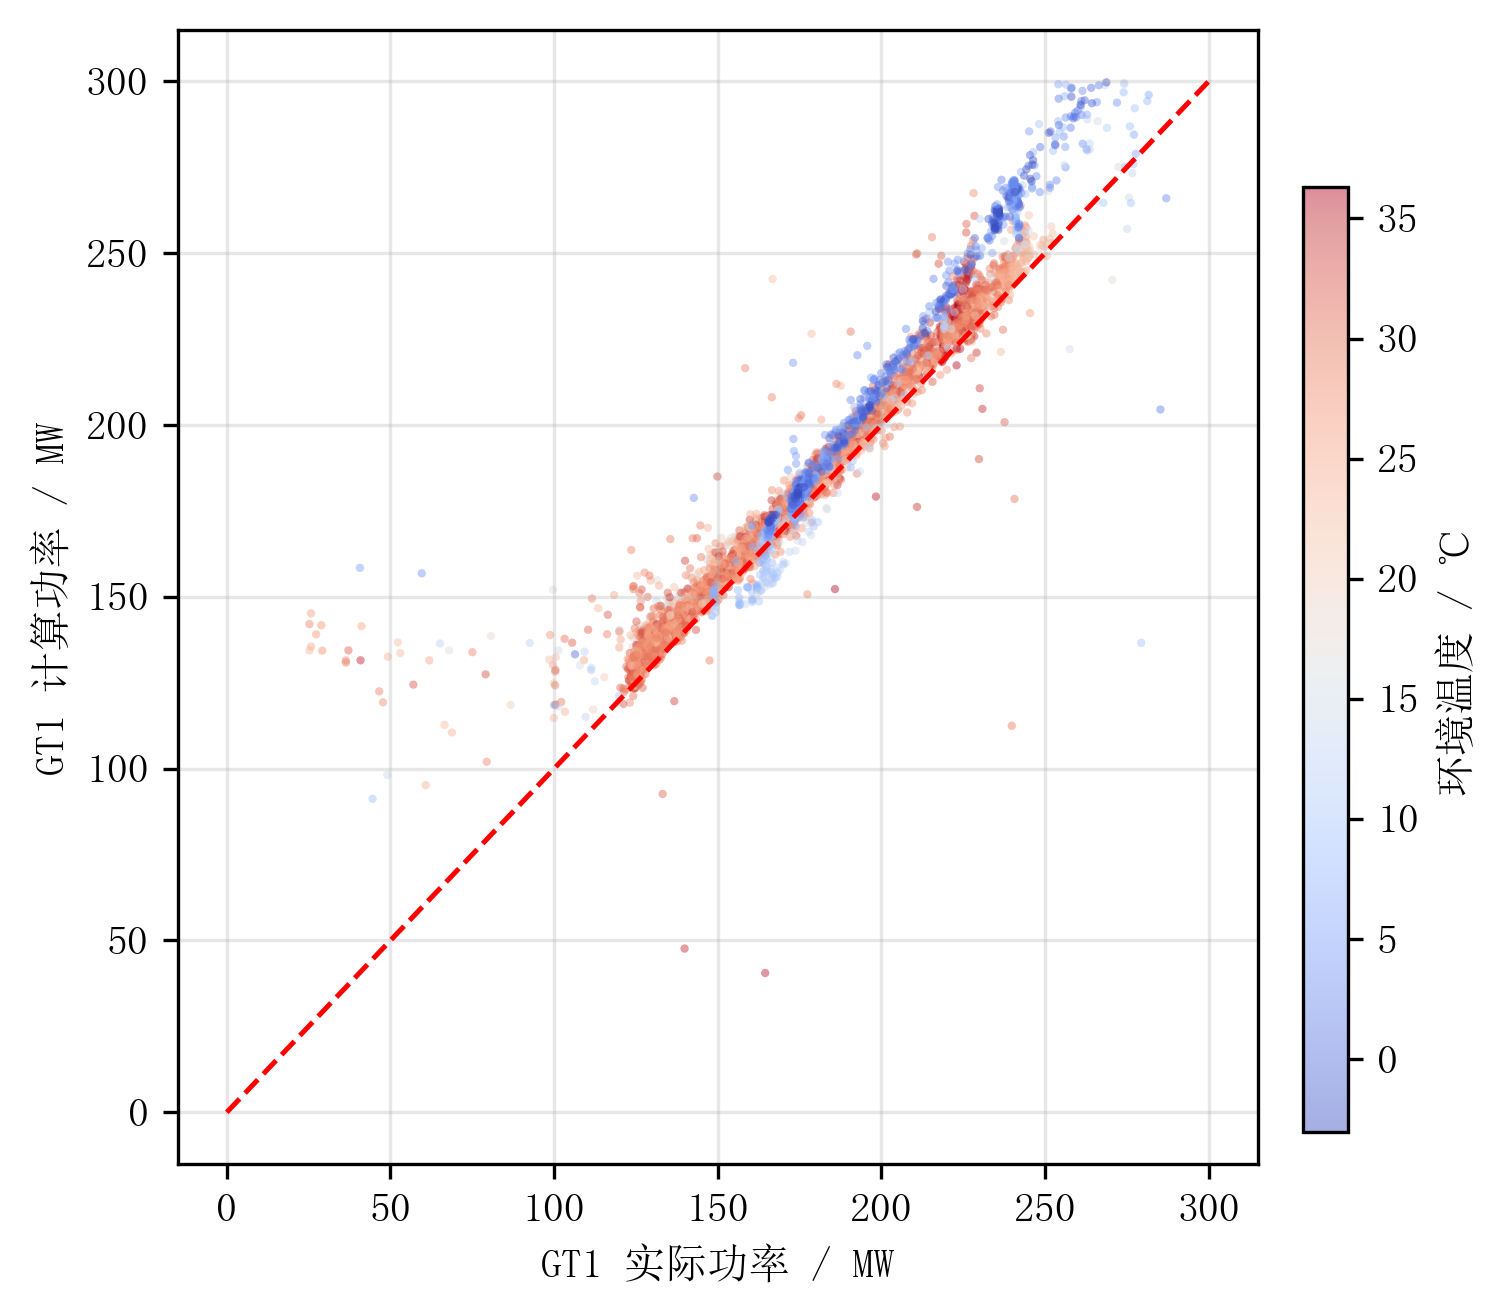
\includegraphics[width=0.8\textwidth]{chapter3/1燃机1出力.png}
  \caption{\#1 燃气轮机出力计算值与实测值对比}
  \label{fig:gt1-air-flow-correction-output}
\end{figure}

\begin{figure}[!htb]
  \centering
  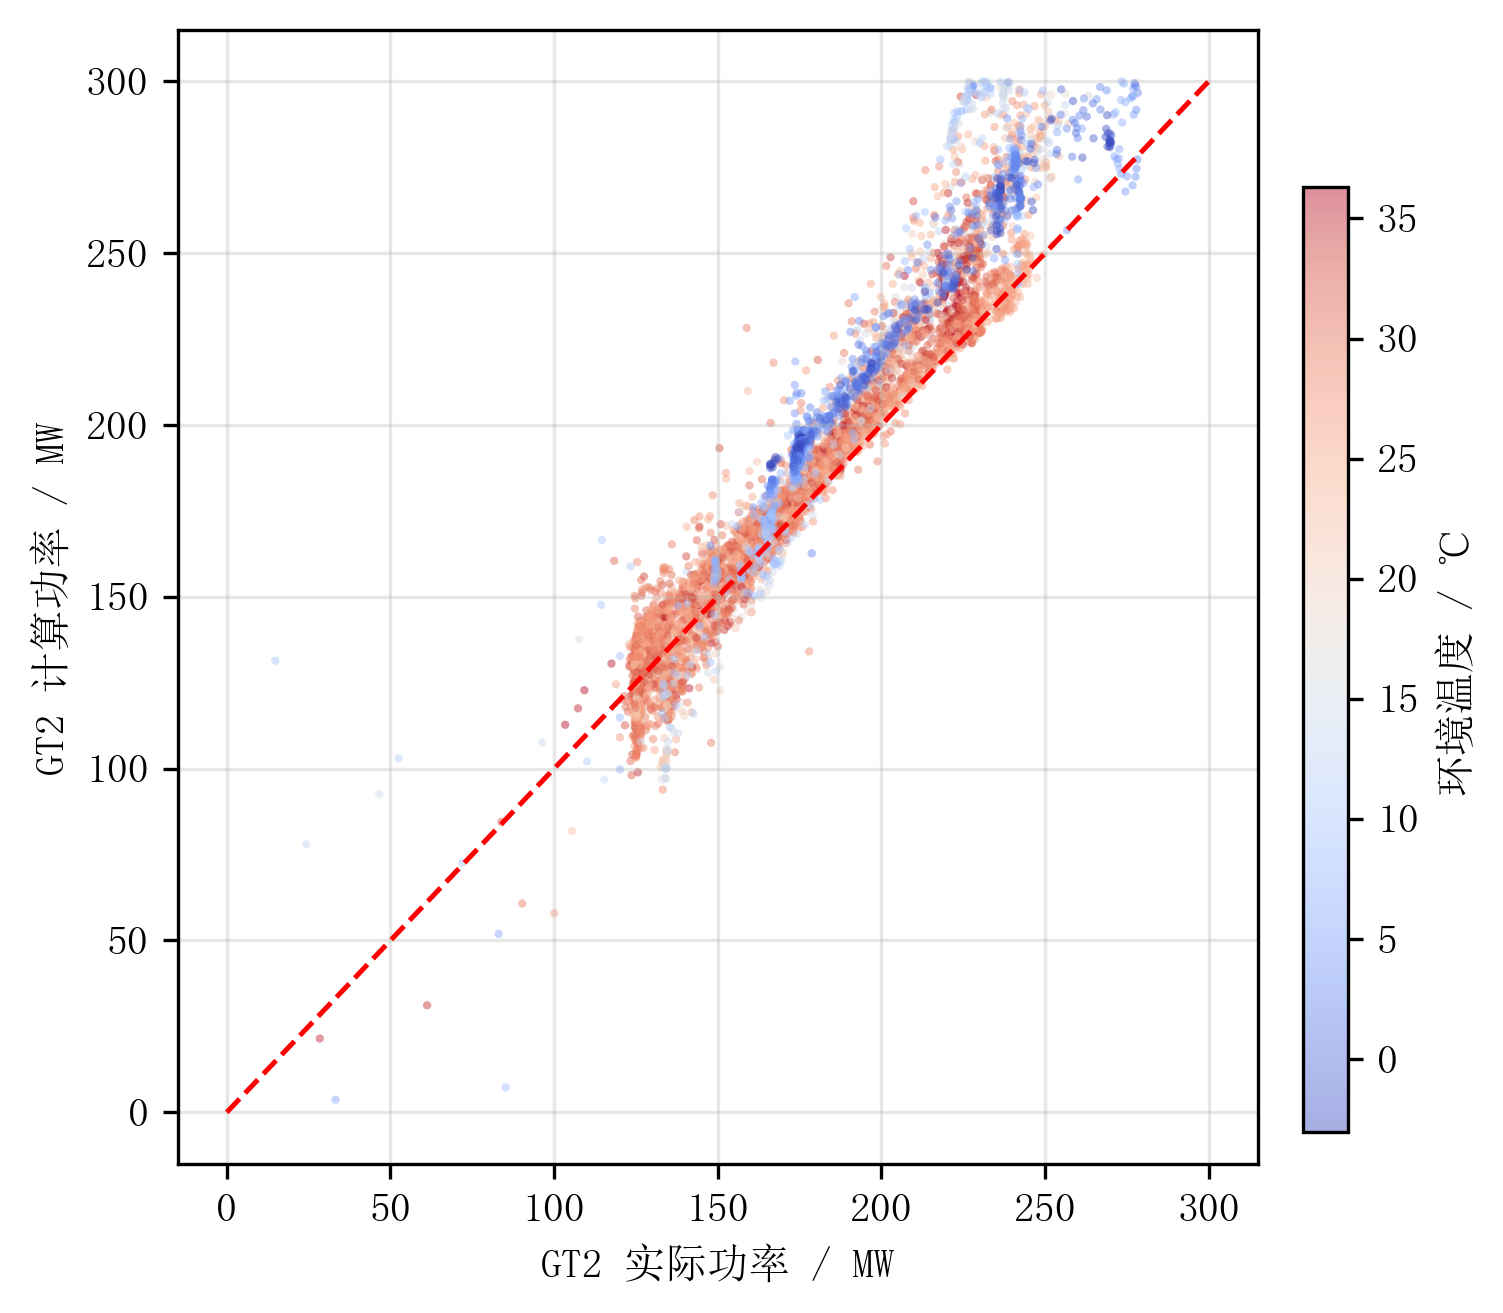
\includegraphics[width=0.8\textwidth]{chapter3/1燃机2出力.png}
  \caption{\#2 燃气轮机出力计算值与实测值对比}
  \label{fig:gt2-air-flow-correction-output}
\end{figure}

\FloatBarrier

\subsection{压气机和透平效率分析}

图~\ref{fig:chapter3-gt1-compressor} 和图~\ref{fig:chapter3-gt2-compressor} 对比了两台燃气轮机压气机的性能计算结果。压气机效率主要反映实际压缩过程相对于等熵压缩过程的接近程度。随着燃气轮机出力升高，压气机通常运行在更接近设计工况的区域，压比和空气流量增加，流动损失相对减小，因而压气机等熵效率整体趋于稳定并保持在较高水平。冬季工况下压气机效率较低，这可能是冬季空气密度较大，体积流量较小，使得压气机偏离设计工况导致的。随燃机出力增大，空气流量相应增大，压气机效率相应升高，这与压气机性能曲线的特性一致。

透平效率反映高温烟气膨胀做功过程的有效程度。透平入口温度、膨胀比、冷却空气掺混比例和排气压力都会影响透平效率。低温环境下机组通常能够在较高负荷或更接近设计匹配的区域运行，透平膨胀比、流量系数及气动匹配状态有所改善，因此计算得到的透平效率相对较高。需要指出的是，实际运行数据中的透平效率由温度、压力、燃料量和烟气流量等测点反算得到，冬季烟气流量修正、比热取值及测点误差也可能对效率结果产生影响。

\begin{figure}[!htb]
  \centering
  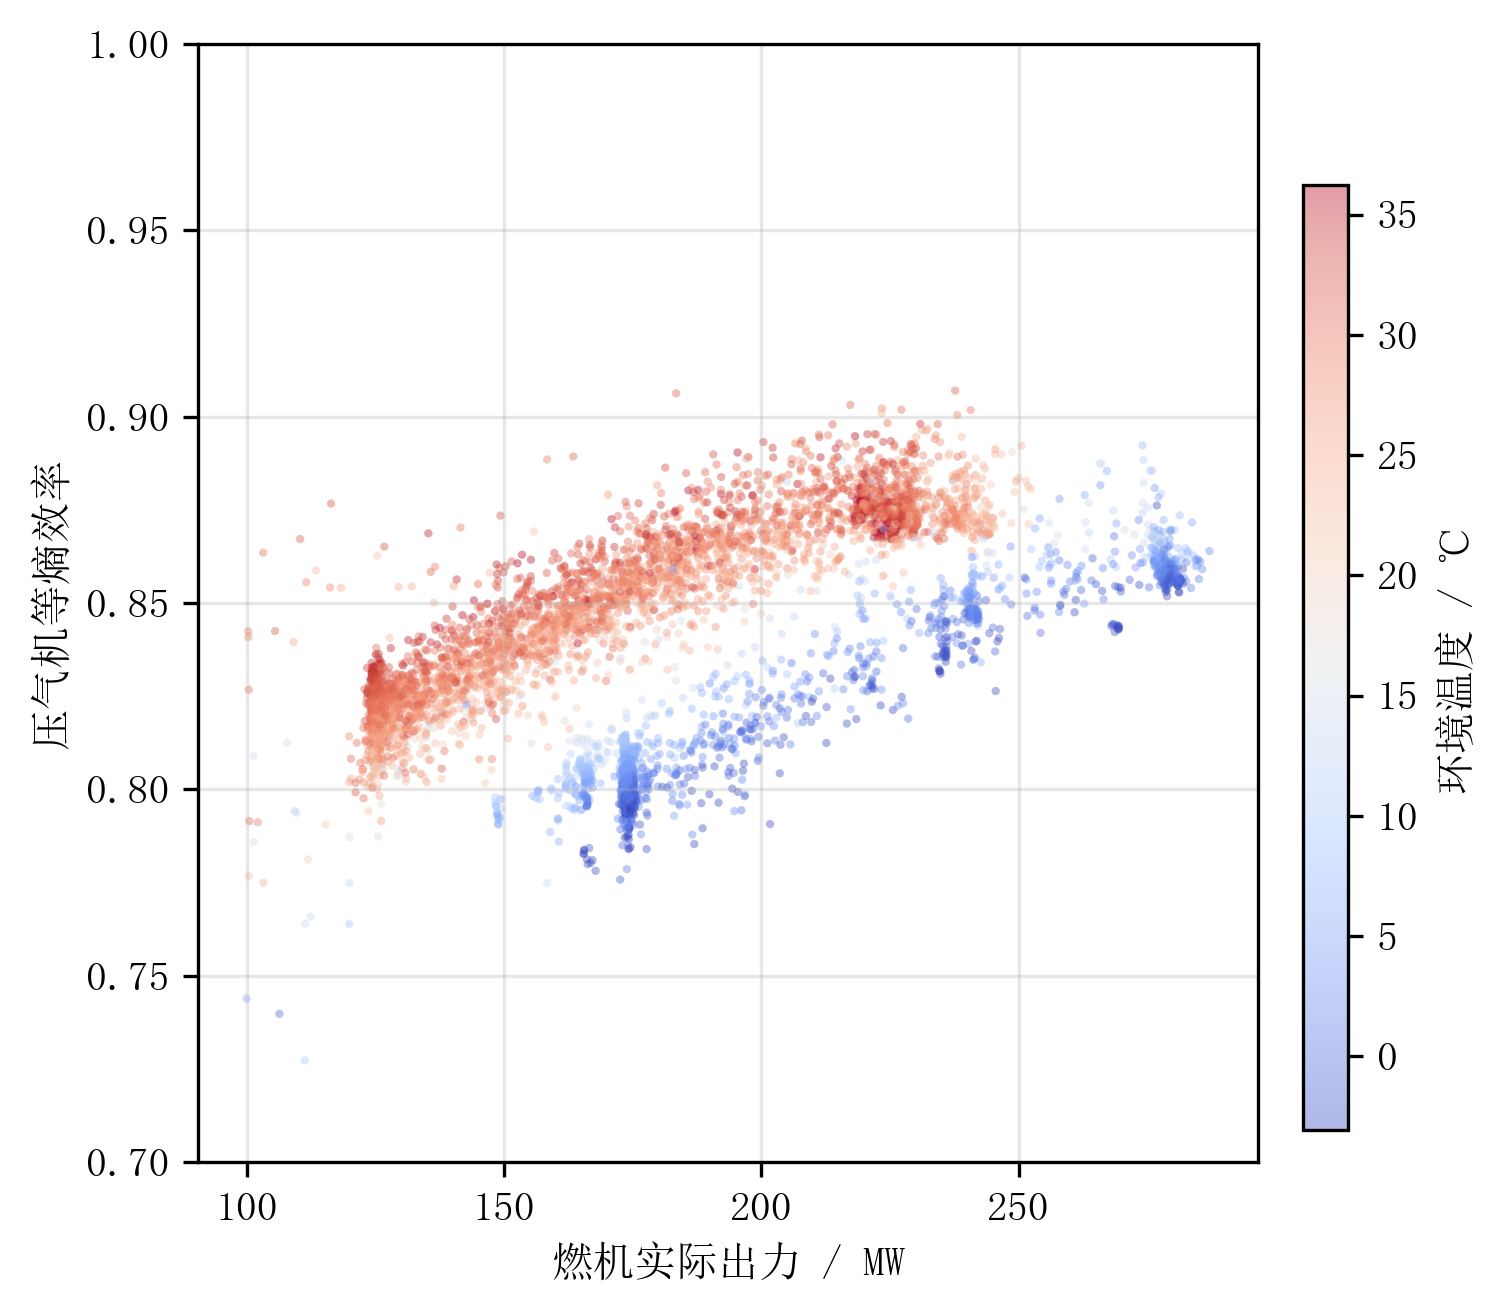
\includegraphics[width=0.8\textwidth]{chapter3/3燃机1压气机.png}
  \caption{\#1 燃气轮机压气机效率}
  \label{fig:chapter3-gt1-compressor}
\end{figure}

\begin{figure}[!htb]
  \centering
  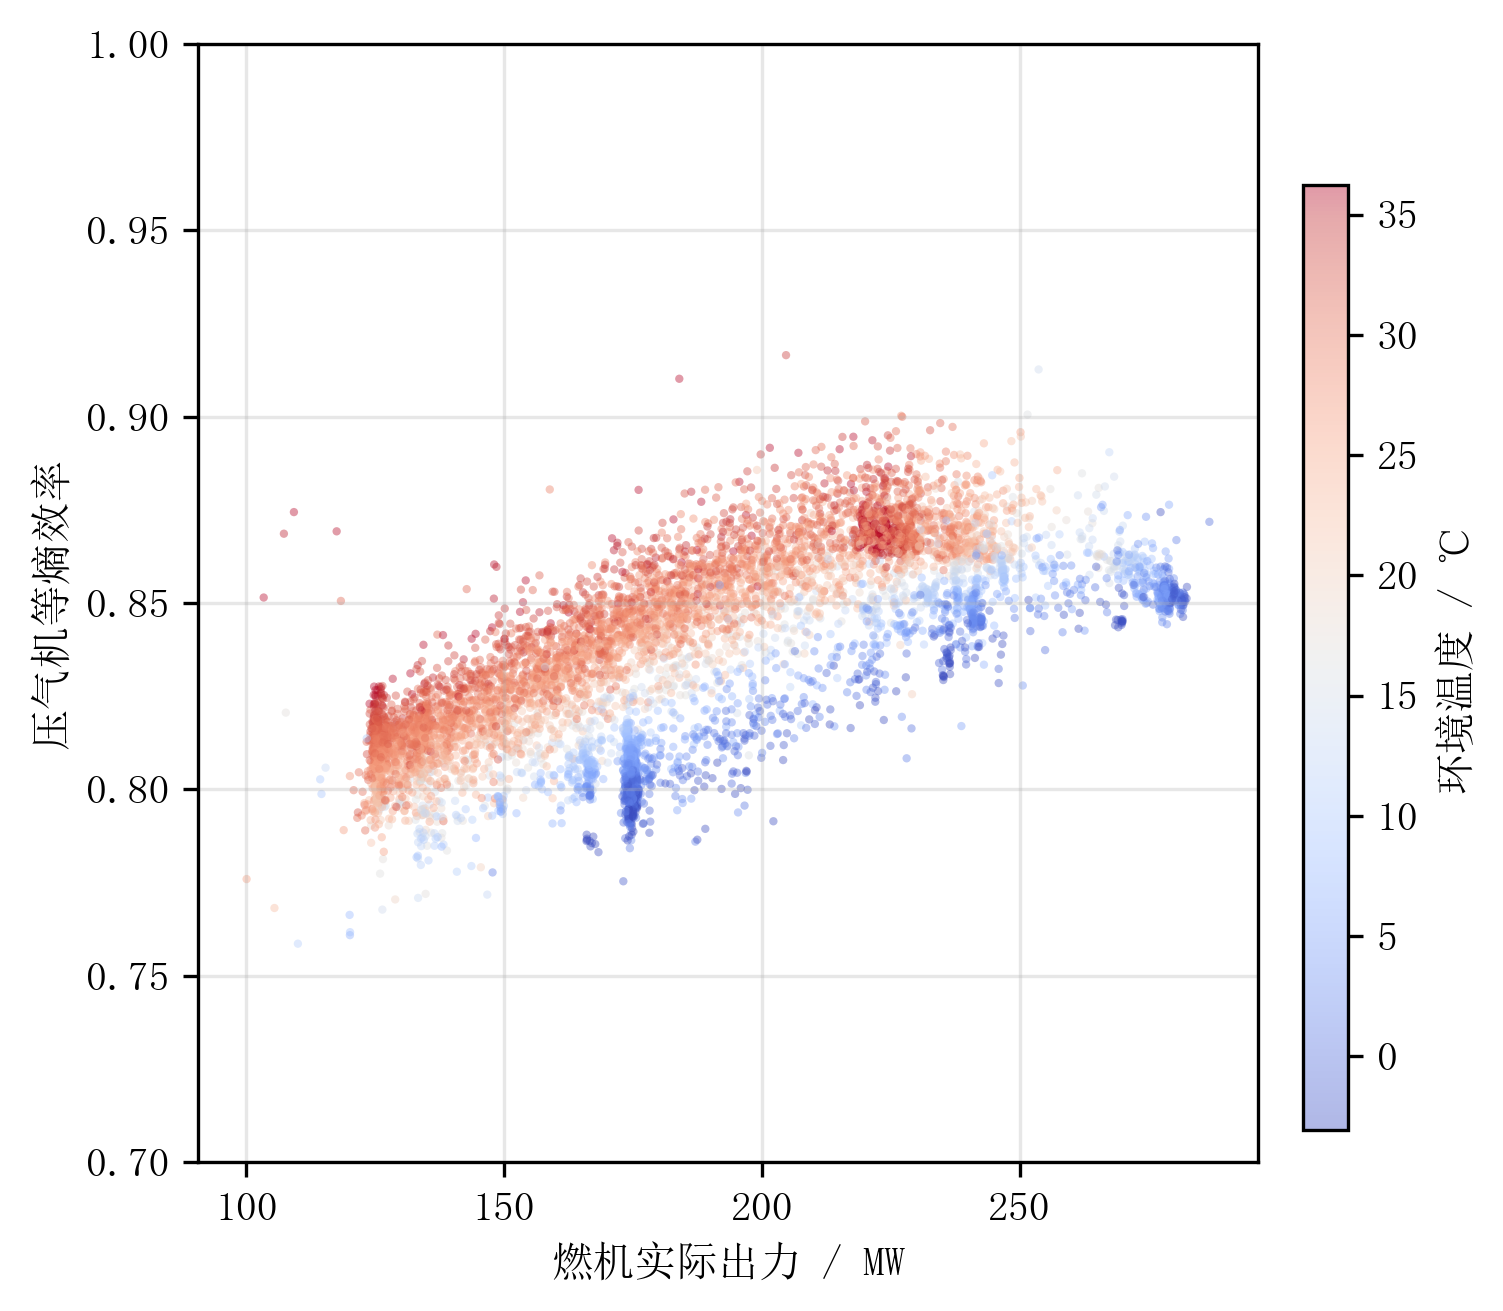
\includegraphics[width=0.8\textwidth]{chapter3/4燃机2压气机.png}
  \caption{\#2 燃气轮机压气机效率}
  \label{fig:chapter3-gt2-compressor}
\end{figure}

\begin{figure}[!htb]
  \centering
  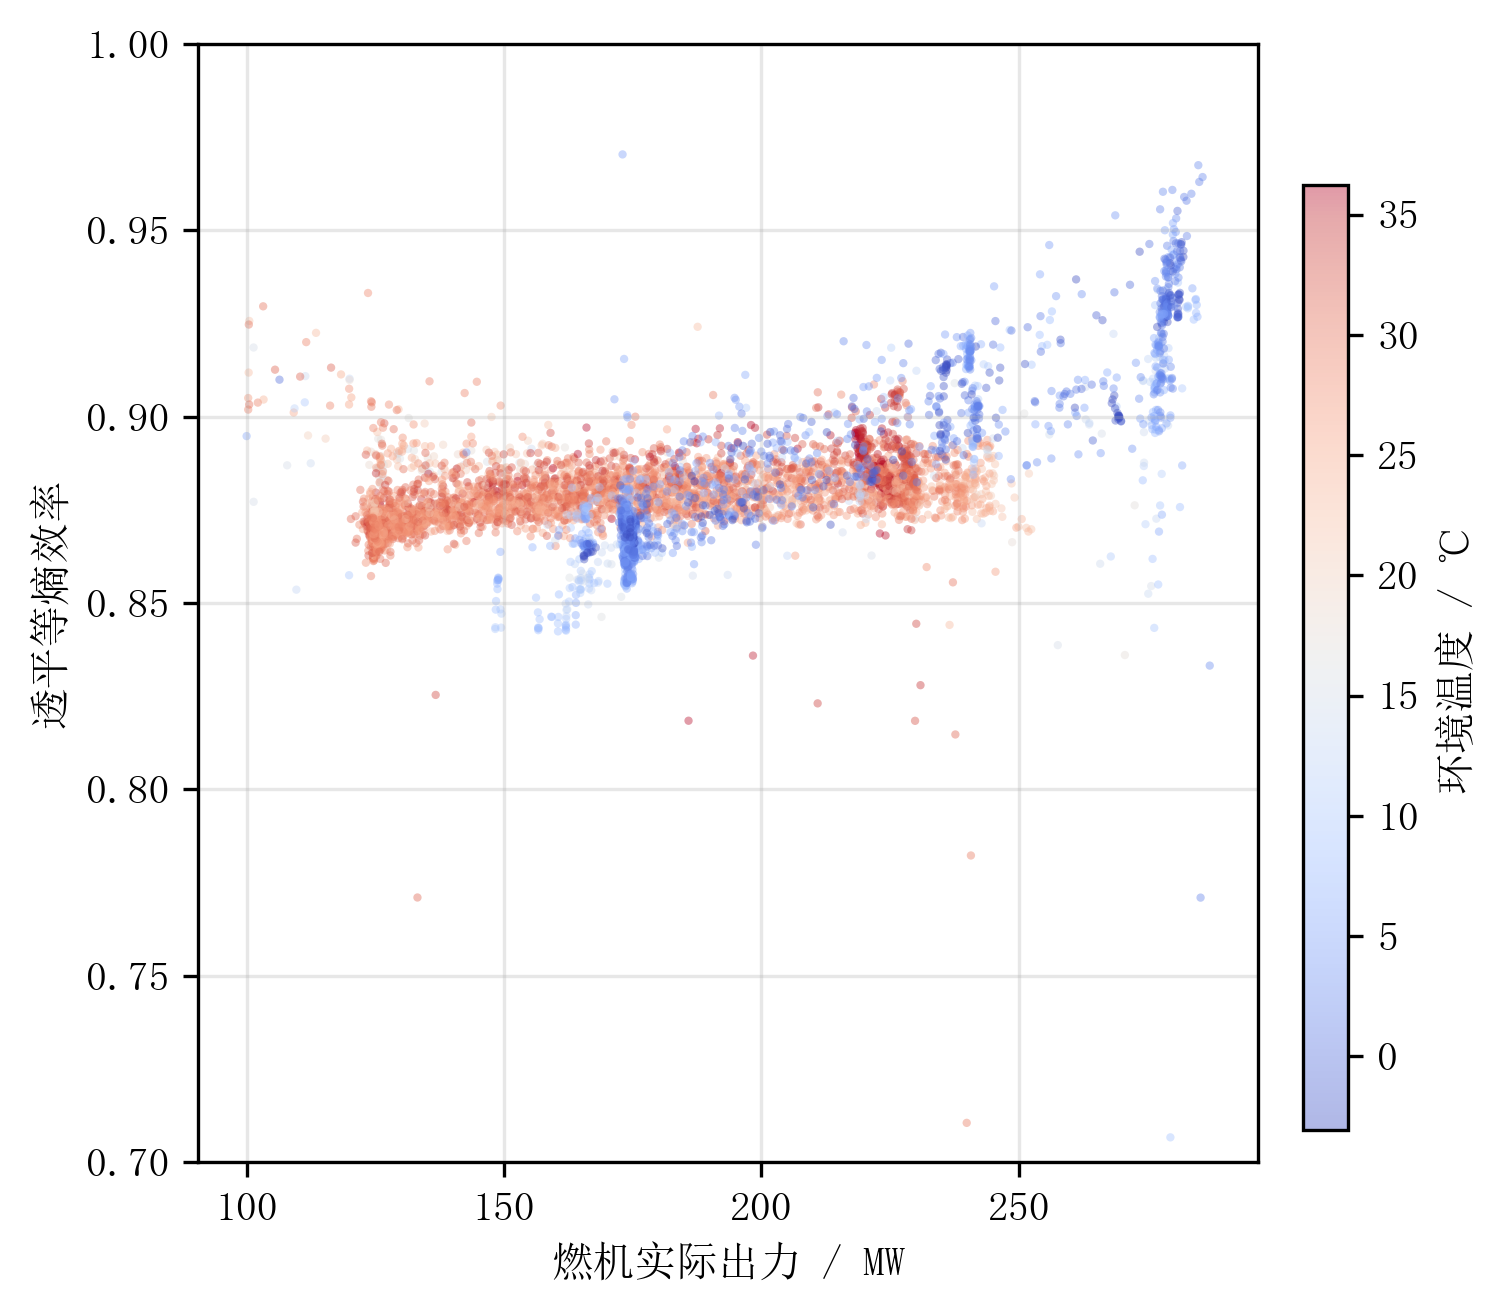
\includegraphics[width=0.8\textwidth]{chapter3/3燃机1透平.png}
  \caption{\#1 燃气轮机透平效率}
  \label{fig:chapter3-gt1-turbine}
\end{figure}

\begin{figure}[!htb]
  \centering
  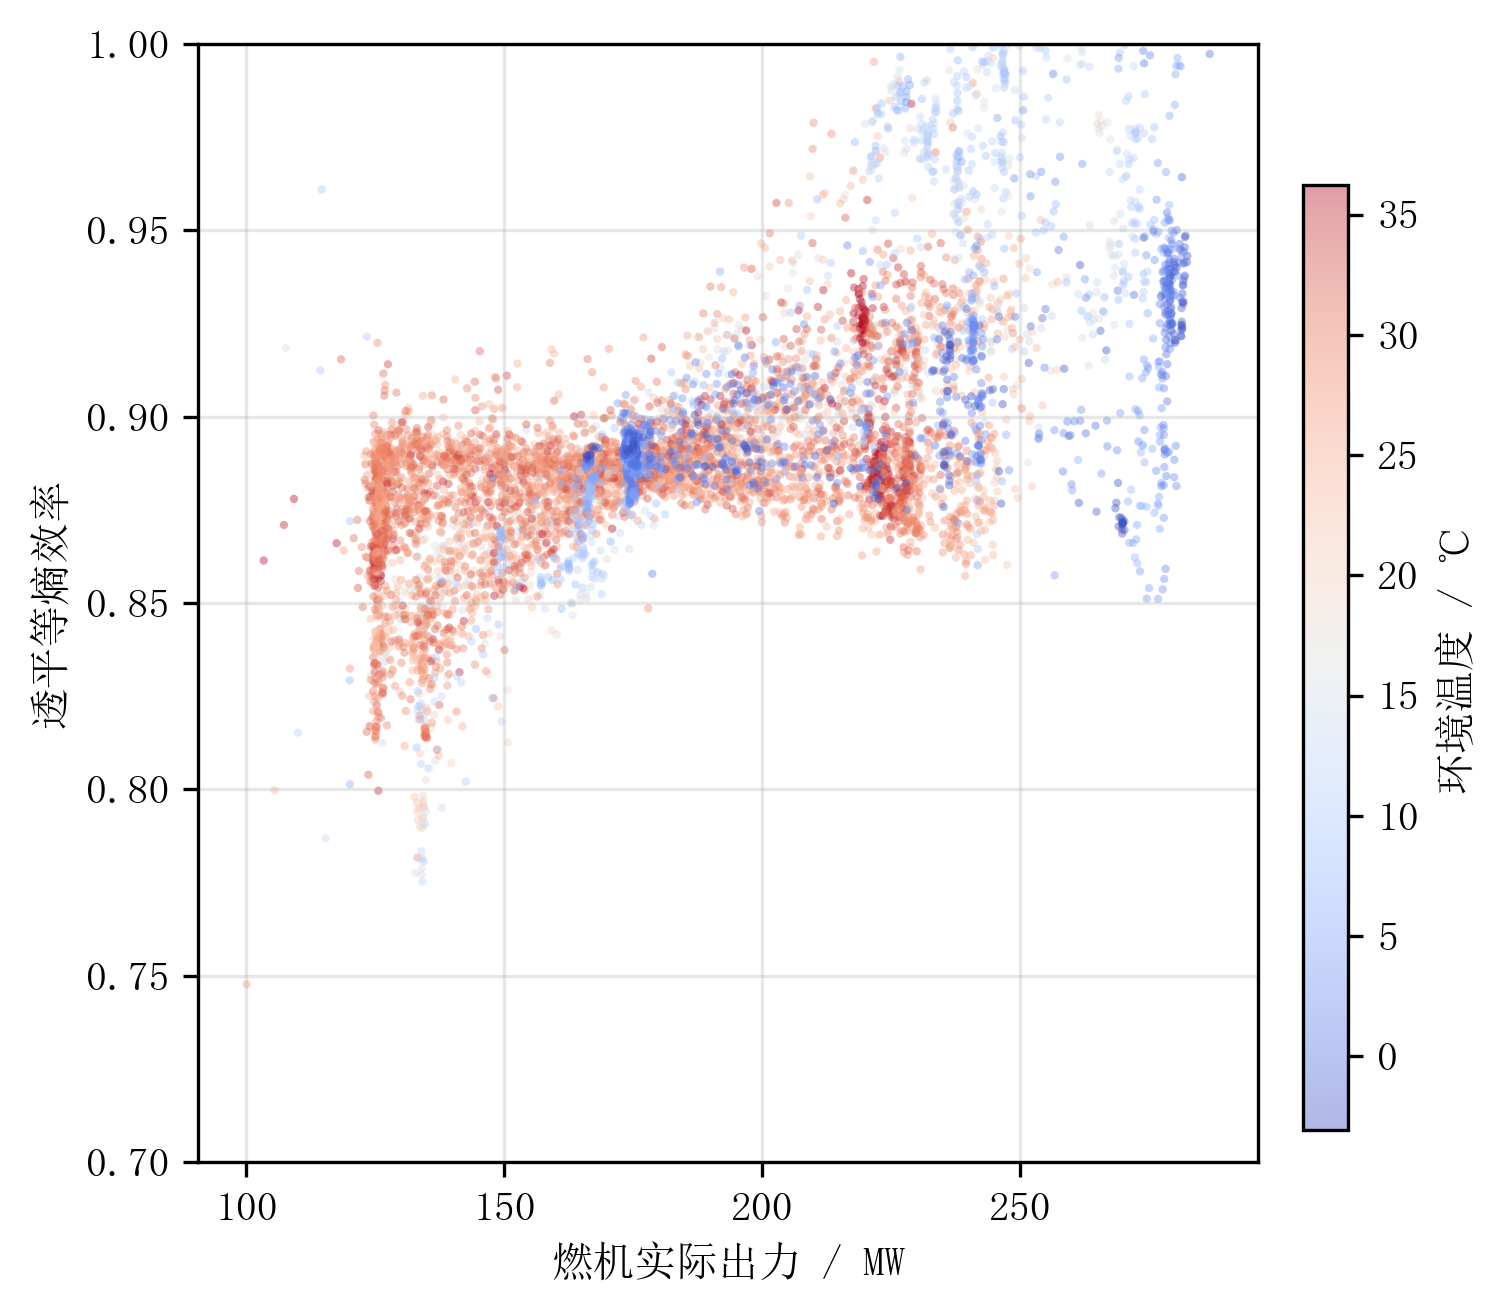
\includegraphics[width=0.8\textwidth]{chapter3/4燃机2透平.png}
  \caption{\#2 燃气轮机透平效率}
  \label{fig:chapter3-gt2-turbine}
\end{figure}

\FloatBarrier

\subsection{燃气轮机能量分配和占比分析}

图~\ref{fig:chapter3-gt1-energy-detail} 和图~\ref{fig:chapter3-gt2-energy-detail} 分别给出了两台燃气轮机的能量分配详情。燃料低位热输入进入燃烧室后，一部分经透平膨胀转化为燃气轮机轴功并由发电机输出，一部分以排气显热形式进入余热锅炉，剩余部分表现为压气机耗功、燃烧室压力损失、透平不可逆损失以及其他散热和机械损失。对于联合循环机组而言，燃气轮机排气能量并非无效损失，而是蒸汽循环的热源。

图~\ref{fig:chapter3-gt1-energy-share} 和图~\ref{fig:chapter3-gt2-energy-share} 进一步给出了燃气轮机能量累计占比随实际出力的变化。发电功率占比约为 $0.28$--$0.36$，且随燃机出力升高略有增加，说明高负荷工况下燃料输入向净输出功的转化比例有所提高；压气机耗功占比约为 $0.38$--$0.43$，是燃气轮机内部功率消耗的主要部分；尾气能量及其他损失占比约为 $0.22$--$0.32$，随出力升高总体略有下降，但仍保留了较高的余热利用潜力。高出力区间部分散点离散程度增大，可能与空气流量测量误差与修正偏差、排气温度波动和测点误差有关。

\begin{figure}[!htb]
  \centering
  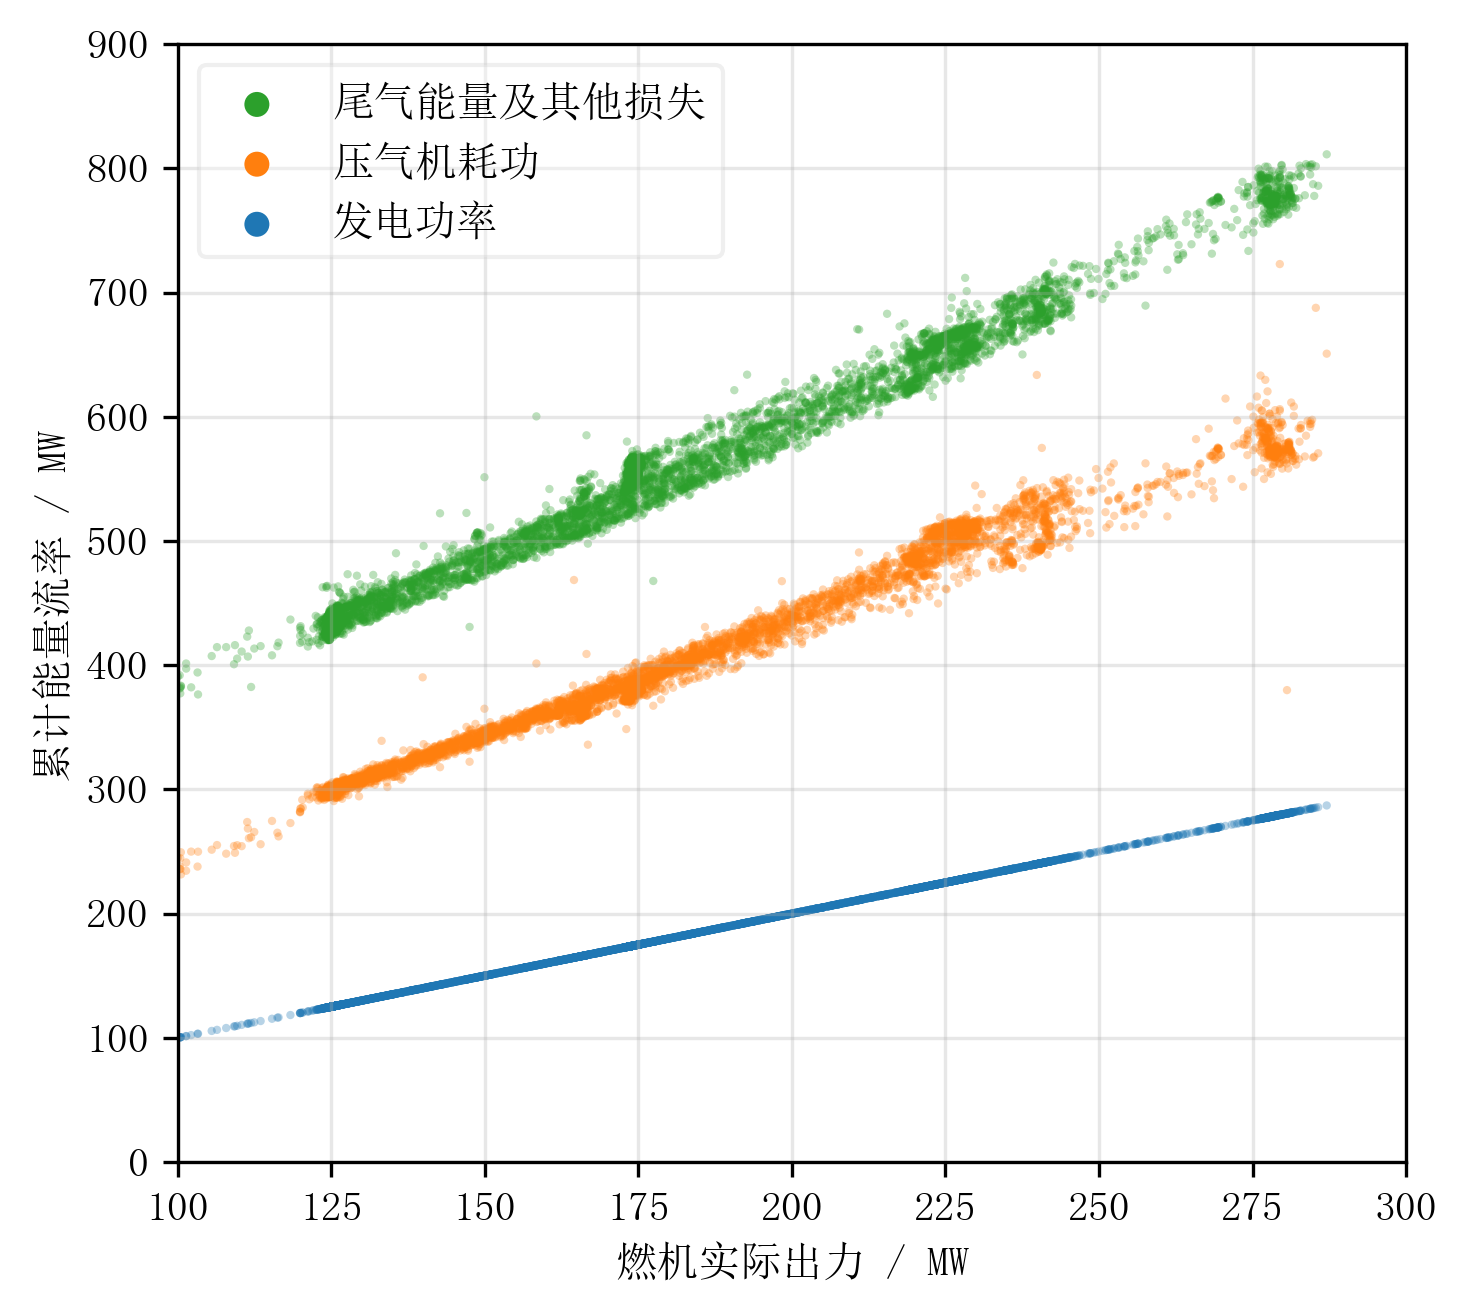
\includegraphics[width=0.8\textwidth]{chapter3/2GT1能量分配.png}
  \caption{\#1 燃气轮机能量分配详情}
  \label{fig:chapter3-gt1-energy-detail}
\end{figure}

\begin{figure}[!htb]
  \centering
  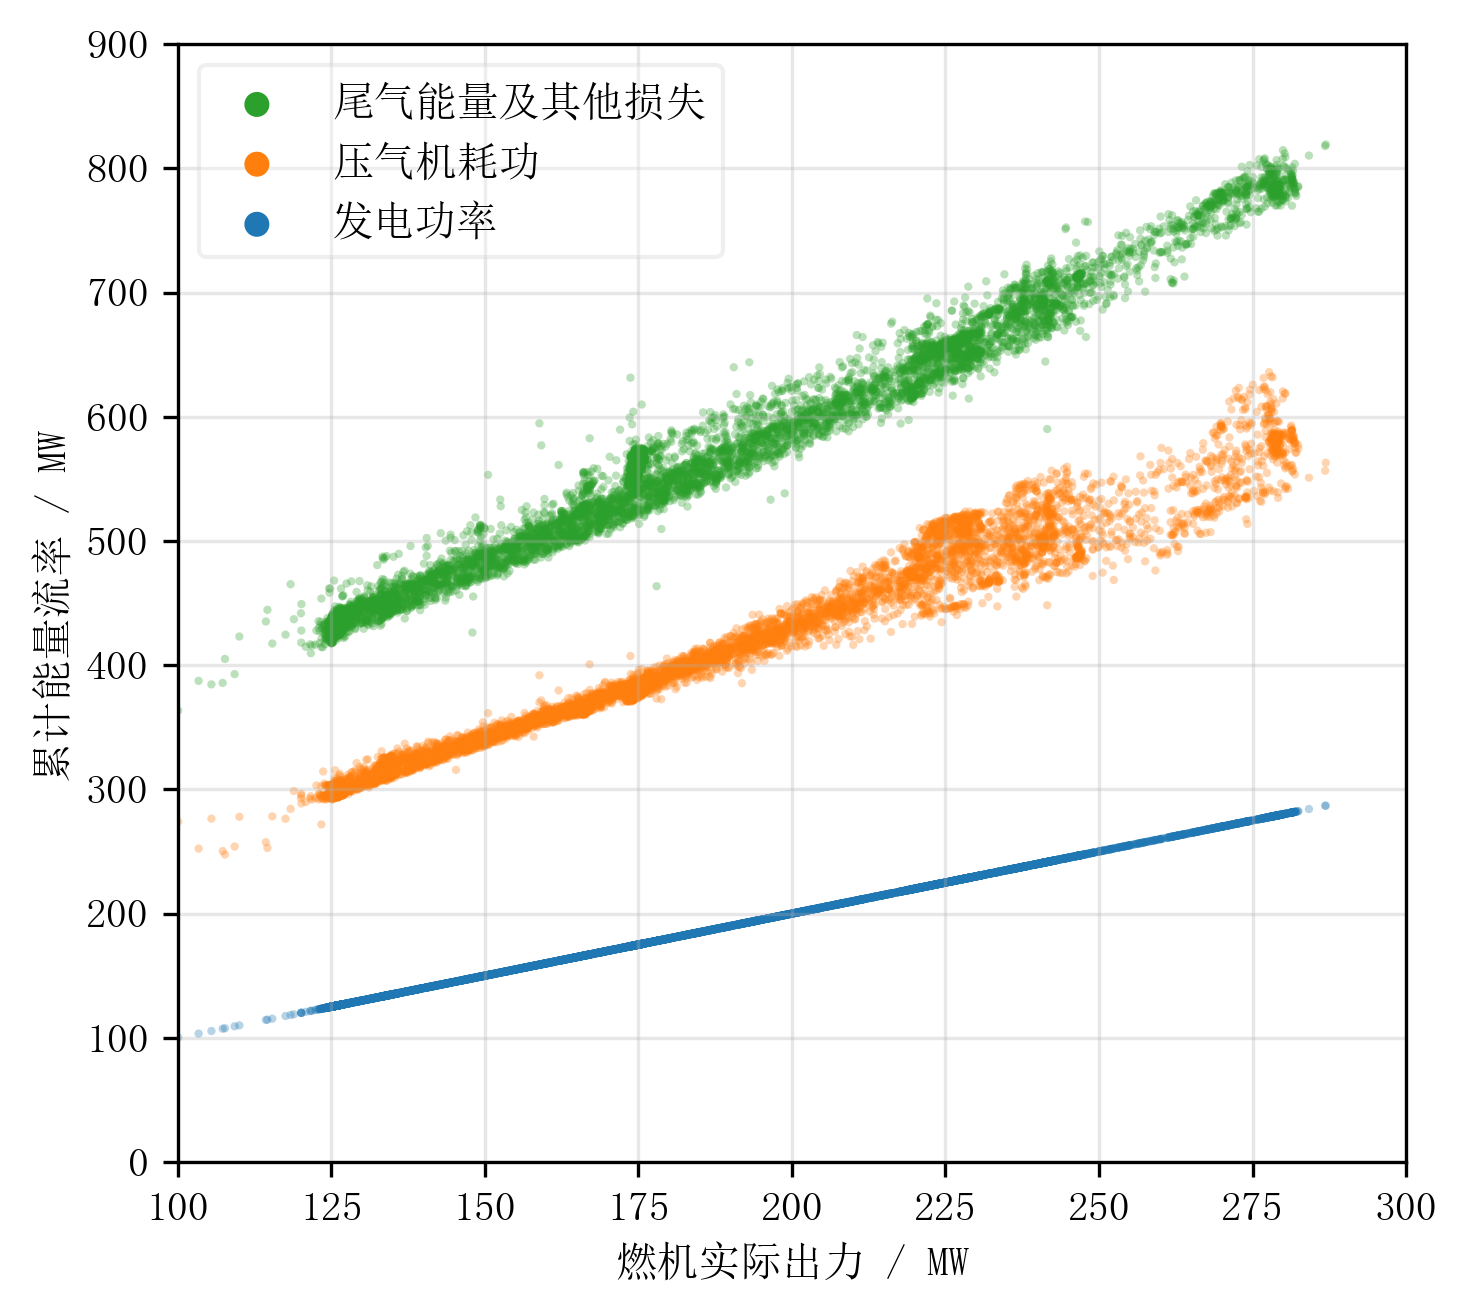
\includegraphics[width=0.8\textwidth]{chapter3/2GT2能量分配.png}
  \caption{\#2 燃气轮机能量分配详情}
  \label{fig:chapter3-gt2-energy-detail}
\end{figure}

\begin{figure}[!htb]
  \centering
  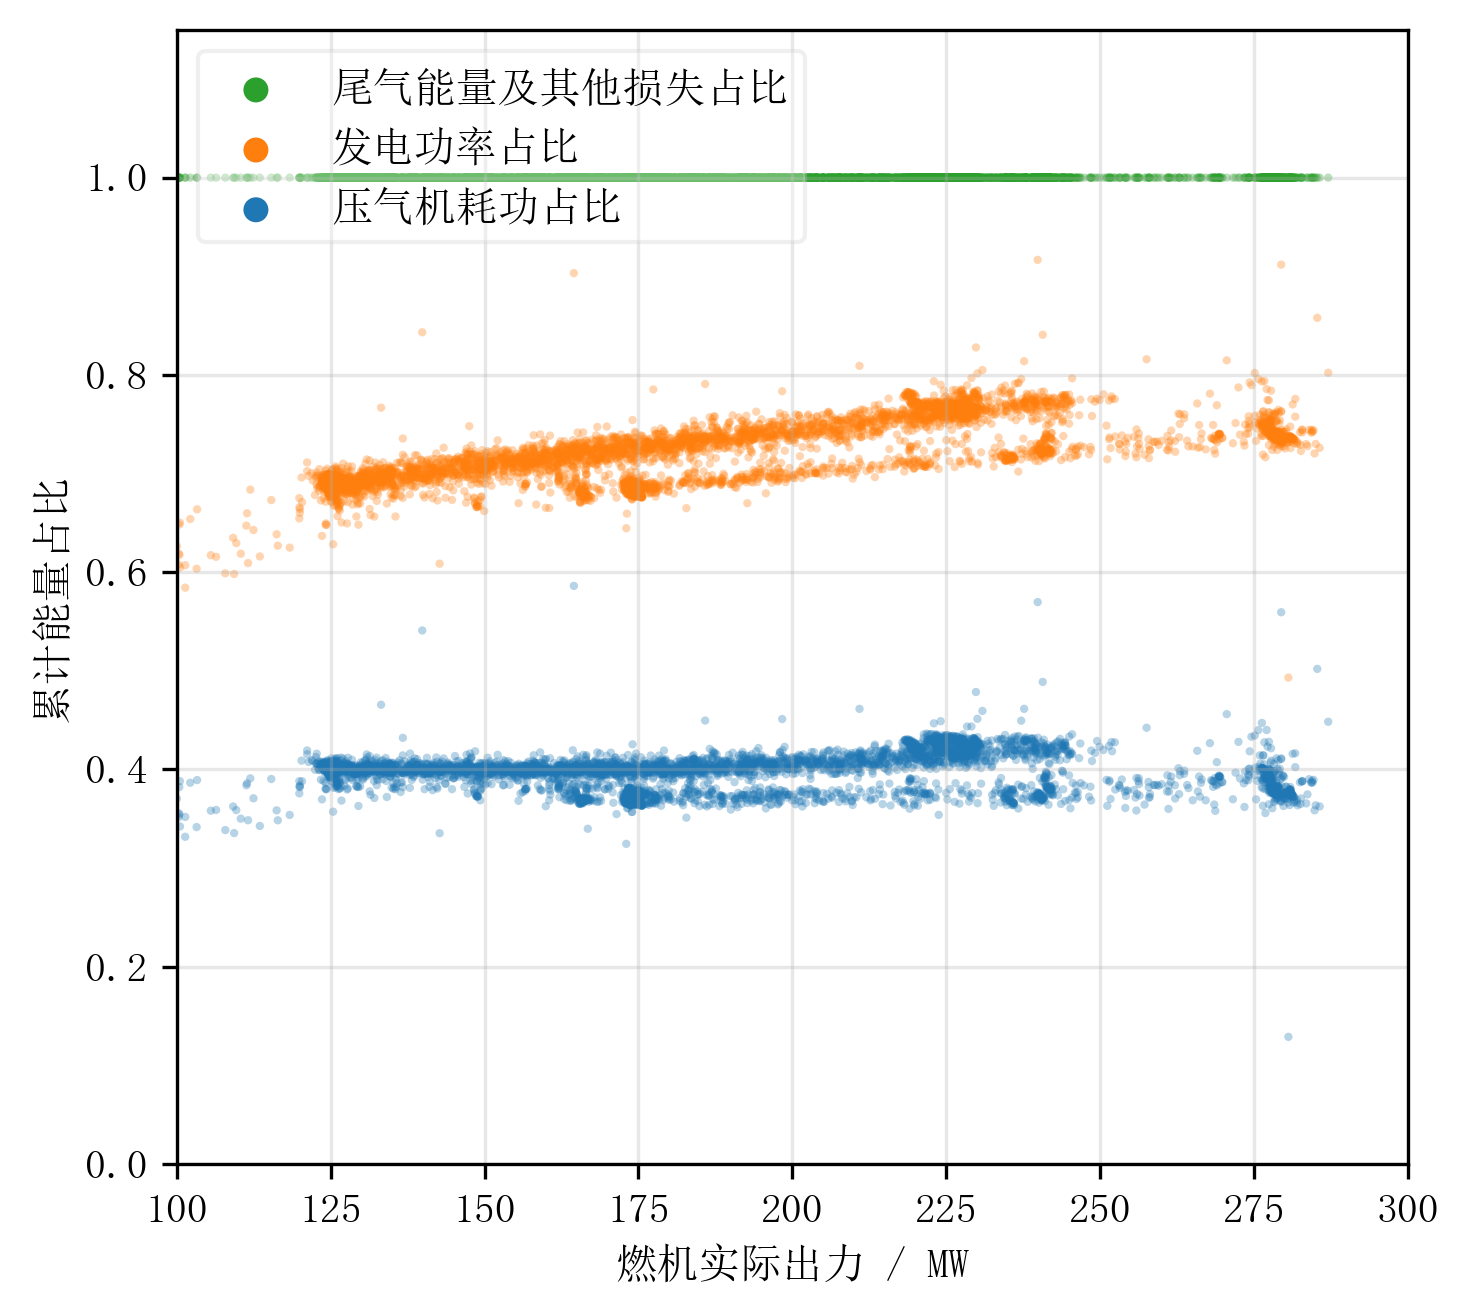
\includegraphics[width=0.8\textwidth]{chapter3/2-1GT1能量占比.png}
  \caption{\#1 燃气轮机能量占比}
  \label{fig:chapter3-gt1-energy-share}
\end{figure}

\begin{figure}[!htb]
  \centering
  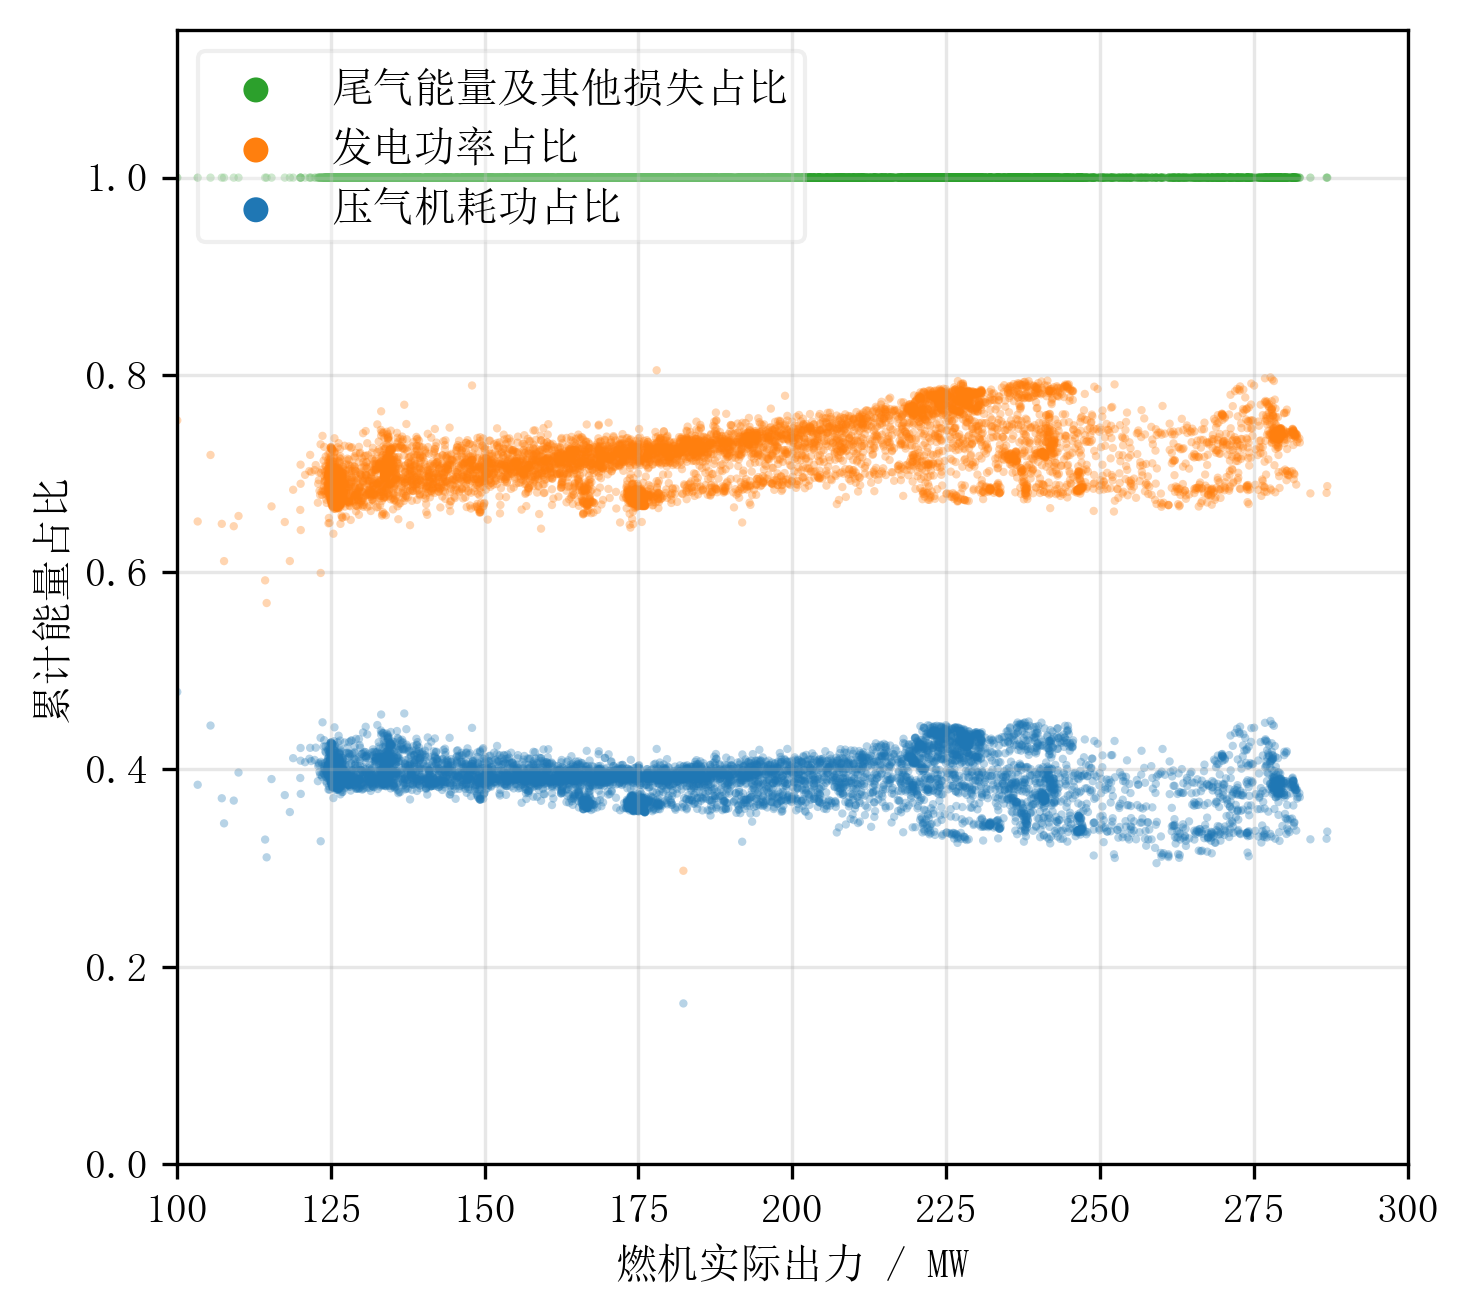
\includegraphics[width=0.8\textwidth]{chapter3/2-1GT2能量占比.png}
  \caption{\#2 燃气轮机能量占比}
  \label{fig:chapter3-gt2-energy-share}
\end{figure}

\FloatBarrier

\section{本章小结}

本章建立了燃气轮机部件级性能分析模型，分别对压气机、燃烧室和透平进行能量分析，并提出基于功率残差的空气流量修正方法。在此基础上，对两台燃气轮机的历史运行工况进行逐点计算，得到空气流量修正效果、部件效率和能量分配等结果。分析结果表明燃气轮机功率计算有较高的精度；压气机和透平效率反映了其在不同负荷下的工况特征；能量分配揭示了燃料输入在发电输出和排气余热之间的分配关系。上述分析为后续余热锅炉、汽轮机以及联合循环整机性能评价提供了燃气轮机侧部件级基础。

\chapter{汽轮机和余热锅炉的建模分析方法}

\section{汽水侧系统建模对象与总体思路}

在燃气--蒸汽联合循环机组中，余热锅炉和汽轮机共同构成蒸汽侧循环。燃气轮机排出的高温烟气进入余热锅炉后，将热量传递给高压、中压和低压汽水系统，产生主蒸汽、再热蒸汽和低压蒸汽；蒸汽进入汽轮机各级缸膨胀做功，随后在凝汽器中凝结，并经凝结水泵、给水泵重新送入余热锅炉。本文在第 2 章所建立的统一流股对象基础上，将汽水侧设备划分为余热锅炉、汽轮机、凝汽器、泵、节流阀和混合器等模块，并通过各模块入口、出口流股的质量流量、焓流率和火用流率计算设备性能指标。

\begin{figure}[htbp]
  \centering
  \fbox{%
    \parbox[c][0.32\textheight][c]{0.82\textwidth}{%
      \centering
      汽水侧设备及流股连接关系示意图预留位置\\[0.6em]
      图中建议绘制两台余热锅炉、高压缸、中压缸、低压缸、凝汽器、
      凝结水泵和给水泵，并标注高压主蒸汽、热再热蒸汽、低压主蒸汽、
      冷再热蒸汽和烟气侧进出口边界。
    }%
  }
  \caption{汽水侧设备及流股连接关系}
  \label{fig:steam-water-system-boundary}
\end{figure}

\section{余热锅炉的建模方法}

余热锅炉是连接燃气轮机排气和蒸汽循环的换热设备。由于测点数量的限制，本文并不逐段建立省煤器、蒸发器、过热器和再热器的详细传热模型，而是从整台余热锅炉的能量输入和输出角度计算其换热性能。对于第 $j$ 台余热锅炉，烟气入口状态记为 $g,\mathrm{in}$，烟气出口状态记为 $g,\mathrm{out}$；汽水侧入口流股集合记为 $\mathcal{W}_{j,\mathrm{in}}$，汽水侧出口流股集合记为 $\mathcal{W}_{j,\mathrm{out}}$。

烟气侧放热功率由入口烟气焓流率与出口烟气焓流率之差表示：
\[
\dot{Q}_{g,j}
=
\dot{m}_{g,\mathrm{in}}h_{g,\mathrm{in}}
-
\dot{m}_{g,\mathrm{out}}h_{g,\mathrm{out}}.
\]
汽水侧吸热功率为所有汽水出口焓流率与入口焓流率之差：
\[
\dot{Q}_{w,j}
=
\sum_{o\in\mathcal{W}_{j,\mathrm{out}}}\dot{m}_o h_o
-
\sum_{i\in\mathcal{W}_{j,\mathrm{in}}}\dot{m}_i h_i.
\]
余热锅炉能量损失可表示为
\[
\dot{Q}_{\mathrm{loss},j}
=
\dot{Q}_{g,j}
-
\dot{Q}_{w,j}.
\]
余热锅炉换热效率采用汽水侧吸热功率与烟气侧放热功率之比表示：
\[
\eta_{\mathrm{HRSG},j}
=
\frac{\dot{Q}_{w,j}}{\dot{Q}_{g,j}}.
\]
同时，为描述烟气在余热锅炉内释放能量占入口烟气总能量的比例，定义换热器有效性为
\[
\varepsilon_{\mathrm{HRSG},j}
=
\frac{\dot{Q}_{g,j}}{\dot{m}_{g,\mathrm{in}}h_{g,\mathrm{in}}}.
\]

在火用分析中，烟气侧释放火用为
\[
\dot{E}_{x,g,j}
=
\dot{m}_{g,\mathrm{in}}e_{x,g,\mathrm{in}}
-
\dot{m}_{g,\mathrm{out}}e_{x,g,\mathrm{out}},
\]
汽水侧吸收火用为
\[
\dot{E}_{x,w,j}
=
\sum_{o\in\mathcal{W}_{j,\mathrm{out}}}\dot{m}_o e_{x,o}
-
\sum_{i\in\mathcal{W}_{j,\mathrm{in}}}\dot{m}_i e_{x,i}.
\]
余热锅炉火用效率定义为汽水侧吸收火用与烟气侧释放火用之比：
\[
\eta_{\mathrm{HRSG},ex,j}
=
\frac{\dot{E}_{x,w,j}}{\dot{E}_{x,g,j}}.
\]
该指标反映烟气高温可用能转化为蒸汽可用能的有效程度。若烟气侧放热功率较高而汽水侧火用增量较低，则说明换热过程中存在较大的传热温差损失或排烟火用损失。

为进一步分析不同压力等级蒸汽的吸热贡献，程序还单独计算高压主蒸汽吸热功率、中压和再热蒸汽吸热功率以及低压主蒸汽吸热功率。高压主蒸汽吸热功率可表示为
\[
\dot{Q}_{\mathrm{HP},j}
=
\dot{H}_{\mathrm{HP,main},j}
-
\dot{H}_{\mathrm{HP,fw},j},
\]
中压和再热蒸汽吸热功率可表示为
\[
\dot{Q}_{\mathrm{IP+RH},j}
=
\dot{H}_{\mathrm{HRH},j}
-
\dot{H}_{\mathrm{IP,fw},j}
-
\dot{H}_{\mathrm{CRH},j},
\]
低压主蒸汽吸热功率则由低压省煤器、低压汽包和低压过热过程的焓流率增量相加得到。上述分项指标用于判断余热锅炉不同压力等级蒸汽对联合循环底循环的贡献。

\section{汽轮机的建模方法}

本文将汽轮机划分为高压缸、中压缸和低压缸三部分进行考虑。两台余热锅炉高压主蒸汽混合后进入高压缸做功，高压缸出口蒸汽与中压主蒸汽混合，再热后进入 中压缸做功；中压缸出口蒸汽与低压主蒸汽混合，进入低压缸做功。在冬季供热工况下，低压蒸汽直接进入热网，不再进入低压缸做功。

对于任一汽轮机缸 $k$，入口状态记为 $\mathcal{F}_{k,\mathrm{in}}$，实际出口状态记为 $\mathcal{F}_{k,\mathrm{out}}$。等熵出口状态记为 $\mathcal{F}_{k,s}$，其定义为
\[
P_{k,s}=P_{k,\mathrm{out}},
\qquad
s_{k,s}=s_{k,\mathrm{in}}.
\]
并得到等熵出口比焓 $h_{k,s}$。

汽轮机缸实际比功为
\[
w_k
=
h_{k,\mathrm{in}}
-
h_{k,\mathrm{out}}.
\]
对应输出功率为
\[
\dot{W}_{k}
=
\dot{m}_{k,\mathrm{out}}
\left(
h_{k,\mathrm{in}}
-
h_{k,\mathrm{out}}
\right).
\]
在稳态无泄漏近似下，$\dot{m}_{k,\mathrm{out}}\approx \dot{m}_{k,\mathrm{in}}$。汽轮机等熵效率定义为实际焓降与等熵焓降之比：
\[
\eta_{k,s}
=
\frac{
h_{k,\mathrm{in}}-h_{k,\mathrm{out}}
}{
h_{k,\mathrm{in}}-h_{k,s}
}.
\]

汽轮机功率计算值由各缸输出功率相加得到：
\[
\dot{W}_{\mathrm{ST,cal}}
=
\dot{W}_{\mathrm{HP}}
+
\dot{W}_{\mathrm{IP}}
+
\dot{W}_{\mathrm{LP}}.
\]
当低压缸进口压力低于设定阈值时，程序将该工况识别为低压缸切缸状态，此时总功率只包括高压缸和中压缸：
\[
\dot{W}_{\mathrm{ST,cal}}
=
\dot{W}_{\mathrm{HP}}
+
\dot{W}_{\mathrm{IP}}.
\]
汽轮机总体等熵效率采用实测汽轮机功率与各缸理想等熵功率之和的比值表示：
\[
\eta_{\mathrm{ST},s}
=
\frac{
\dot{W}_{\mathrm{ST,act}}
}{
\dot{W}_{\mathrm{HP},s}
+
\dot{W}_{\mathrm{IP},s}
+
\dot{W}_{\mathrm{LP},s}
},
\]
其中，各缸理想等熵功率为
\[
\dot{W}_{k,s}
=
\dot{m}_{k,\mathrm{in}}
\left(
h_{k,\mathrm{in}}
-
h_{k,s}
\right).
\]

\section{凝汽器、泵和辅助部件的建模方法}

凝汽器用于将低压缸排汽凝结为凝结水，并将蒸汽余热排向冷端。本文程序将凝汽器视为一个单入口、单出口设备，入口为低压缸出口，出口为凝汽器出口。凝汽器放热功率由入口和出口焓流率之差计算：
\[
\dot{Q}_{\mathrm{cond}}
=
\dot{m}_{\mathrm{cond,in}}h_{\mathrm{cond,in}}
-
\dot{m}_{\mathrm{cond,out}}h_{\mathrm{cond,out}}.
\]
该指标反映低压缸排汽在凝汽器中的冷凝放热量，同时也影响凝汽器真空和低压缸排汽状态。

泵模型用于描述凝结水泵、高压给水泵和中压给水泵等加压设备。对于任一泵 $p$，入口状态记为 $\mathcal{F}_{p,\mathrm{in}}$，实际出口状态记为 $\mathcal{F}_{p,\mathrm{out}}$。等熵出口状态 $\mathcal{F}_{p,s}$ 满足
\[
P_{p,s}=P_{p,\mathrm{out}},
\qquad
s_{p,s}=s_{p,\mathrm{in}}.
\]
泵实际比功为
\[
w_p
=
h_{p,\mathrm{out}}
-
h_{p,\mathrm{in}},
\]
输入功率为
\[
\dot{W}_{p}
=
\dot{m}_{p,\mathrm{out}}
\left(
h_{p,\mathrm{out}}
-
h_{p,\mathrm{in}}
\right).
\]
泵等熵效率定义为等熵压缩比焓升与实际比焓升之比：
\[
\eta_{p,s}
=
\frac{
h_{p,s}-h_{p,\mathrm{in}}
}{
h_{p,\mathrm{out}}-h_{p,\mathrm{in}}
}.
\]

节流阀主要用于描述低压汽包给水调节阀等节流过程。程序计算节流阀压力降和比焓变化：
\[
\Delta P_{\mathrm{tv}}
=
P_{\mathrm{in}}-P_{\mathrm{out}},
\]
\[
\Delta h_{\mathrm{tv}}
=
h_{\mathrm{out}}-h_{\mathrm{in}}.
\]
理想绝热节流过程中比焓近似不变，因此 $\Delta h_{\mathrm{tv}}$ 可用于检查测点和流股构造的一致性。

混合器用于描述多股汽水流股混合过程，主要包括各股蒸汽合并，以及减温器冷却等。混合过程质量和能量守恒，但存在混合火用损失。

\[
\dot{m}_{m,\mathrm{out}}
=
\sum_{i\in\mathcal{F}_{m,\mathrm{in}}}
\dot{m}_i .
\]

\[
\sum_{i\in\mathcal{F}_{m,\mathrm{in}}}
\dot{m}_i h_i
=
\dot{m}_{m,\mathrm{out}}h_{m,\mathrm{out}} .
\]

\[
\dot{E}_{x,\mathrm{dest},m}
=
\sum_{i\in\mathcal{F}_{m,\mathrm{in}}}
\dot{m}_i e_{x,i}
-
\dot{m}_{m,\mathrm{out}}e_{x,m,\mathrm{out}} .
\]

\section{汽水侧性能分析}


\chapter{燃气蒸汽联合循环建模分析方法}
\chapter{结论与展望}

\section{研究工作总结}

本文围绕某二拖一燃气-蒸汽联合循环热电联产机组，基于历史运行数据建立了燃气轮机、余热锅炉、汽轮机以及联合循环整机的性能分析模型，并从能量分析和相关性分析两个层面对机组运行特性进行了研究。主要工作和结论如下。

首先，本文建立了统一的工质流股建模方法。针对联合循环机组中空气、天然气、烟气、水和水蒸气等多类工质并存的问题，本文将工质状态统一表示为包含温度、压力、质量流量、组分、比焓、比熵和比㶲等参数的流股对象。该方法使不同设备之间的质量流和能量流能够连续传递，为后续部件模型和整机模型提供了统一的数据基础。

其次，本文建立了燃气轮机部件级性能分析模型。将压气机、燃烧室和透平分别作为控制体，计算压气机耗功和等熵效率，燃烧室燃料热输入、出口烟气状态，以及透平输出功、等熵效率和等熵损失功率。结果表明，各个计算值具有较高的精度，能够较好地反映燃气轮机的运行状态和性能水平。

再次，本文建立了余热锅炉和汽轮机的汽水侧性能分析模型。余热锅炉模型从整台设备的烟气侧放热和汽水侧吸热出发，计算换热效率、烟气能量释放、水侧吸热分配以及不同压力等级蒸汽的热量贡献。汽轮机模型将高压缸、中压缸和低压缸分别建模，计算各缸输出功率和等熵效率，并考虑供热工况下低压蒸汽进入热网导致的通流方式变化。结果表明，余热锅炉高压蒸汽吸热和汽轮机高、中压缸出力是底循环发电能力的重要来源；供热工况下，部分蒸汽能量由发电侧转移至热网侧，使汽轮机出力和热电效率之间呈现不同于非供热工况的变化规律。

最后，本文对联合循环效率影响因素进行了相关性分析。非供热工况下，联合循环发电效率与汽机出力、整机负荷、主蒸汽参数和余热回收能力密切相关，说明提高燃气轮机高效运行水平和增强蒸汽循环做功能力是提升发电效率的关键。供热工况下，热电效率与供热量、环境条件和燃机总出力关系更为密切，表明供热需求和季节性环境变化会显著改变机组能量分配方式。相关性分析还表明，多数运行参数之间存在明显耦合关系，效率优化需要结合部件热力模型进行综合判断，不能仅依据单一变量变化作出结论。

总体而言，本文建立的模型能够基于运行数据对联合循环机组进行部件级和整机级性能评价，较好地反映燃气轮机、余热锅炉、汽轮机和供热系统之间的能量耦合关系。研究结果可为热电联产机组的运行诊断、性能评价和运行优化提供参考，并有望应用到实际电厂的在线性能监测和运行优化系统中。

\section{未来工作展望}

本文研究仍存在一些不足，后续可从以下几个方面进一步完善。

第一，空气流量测点的偏差较大，对后续压气机和透平的性能计算也产生一定影响，需要寻找更可靠的修正方法。后续可进一步引入环境参数、负荷水平和设备运行状态等变量，建立更具泛化能力的空气流量修正模型；同时，可结合燃气轮机功率平衡关系反算空气流量，以提高缺失测点条件下质量流量边界的可靠性。

第二，可进一步细化余热锅炉和汽轮机模型。本文仅从整台余热锅炉的能量输入输出角度分析换热性能，尚未对省煤器、蒸发器、过热器和再热器等各段换热器分别建模，也未充分考虑给水泵、汽包、减温器和节流阀等辅助设备对系统性能的影响。初步分析表明，减温器混合过程引起的不可逆损失较为显著，通过优化减温水调节策略有望提高整机运行效率。后续可建立更精细的分段换热模型，分析不同工况下各换热器的传热特性及其对机组性能的影响，为设备改造和运行优化提供更具针对性的指导。

第三，影响因素分析有待深化。本文采用 Pearson 相关系数识别了与效率变化关联最强的运行参数，但尚未深入区分各变量之间的耦合关系。后续仍需结合部件级热力模型和多变量分析方法，进一步辨识关键参数对效率变化的独立影响及其可调节路径。

第四，可开展面向运行优化的工况寻优研究。本文主要完成性能计算和影响因素分析，后续可在此基础上建立以发电效率、热电效率、供热量或燃料消耗量为目标的优化模型，研究燃气轮机负荷分配、供热抽汽量、主蒸汽参数和余热锅炉运行边界的协同优化方法，为实际运行调度提供更直接的决策支持。

综上，本文的研究构建起了基于运行数据的联合循环机组性能分析框架，并揭示了机组运行特性和效率影响因素。后续工作将进一步完善模型细节，深入分析影响机理，并开展面向优化的工况寻优研究，以期为热电联产机组的高效运行提供更全面的理论支持和实践指导。


% ======================
% 参考文献
% ======================
\cleardoublepage
\addcontentsline{toc}{chapter}{参考文献}

\bibliographystyle{gbt7714-numerical}
\bibliography{references}

\end{document}